\newpage

\section{Path Planning on Real-world Maps}

We have collected three real-world occupancy grid maps produced by SLAM sensors and converted them into internal maps. The maps have been used in the following works: \cite{first_map}, \cite{second_map} and \cite{third_map}.

Figures \ref{fig: wp_vs_a_1}, \ref{fig: wp_vs_a_2} and \ref{fig: wp_vs_a_3} highlight the performance of the Global Way-point LSTM Planner against A* on the real-world maps. Some runs achieve great results while others completely fail (in the sense that we fail to place the last global way-point on the goal). Furthermore, we can notice that the algorithm maintains the same behaviour across different environments which confirms the robustness to unknown environments property. This is intuitively correct, as we have used Machine Learning methods to find the path, and thus, we inherit the generalisation properties.

It should be noted that the run-times where significantly higher for the Global Way-point LSTM Planner due to the parallelising issue. We have also varied the global kernel max iterations to highlight the importance of choosing a proper argument. As a general rule, the number of iterations should be proportional to the size of the map.

\pagebreak

\begin{figure}[]
  \centering
  \begin{subfigure}[b]{0.48\linewidth}
    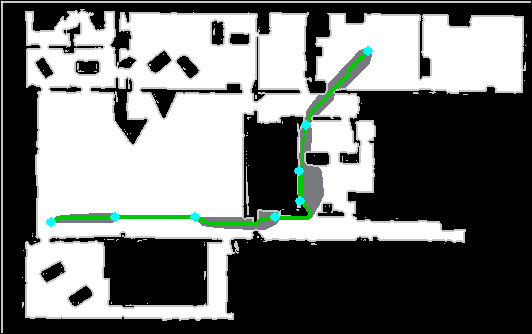
\includegraphics[width=\linewidth]{images/screenshot_134.png}
     \caption{Global Way-point LSTM Planner (max iterations 80)}
  \end{subfigure}
  \hfill
  \begin{subfigure}[b]{0.48\linewidth}
    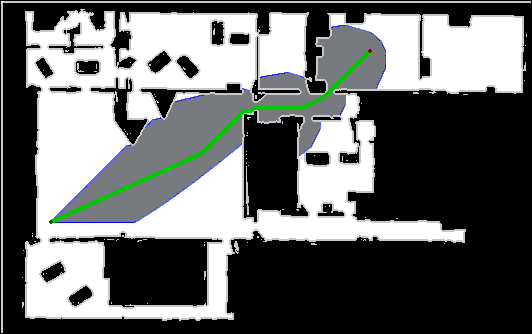
\includegraphics[width=\linewidth]{images/screenshot_107.png}
     \caption{A*\newline}
  \end{subfigure}
  \hfill
  \begin{subfigure}[b]{0.48\linewidth}
    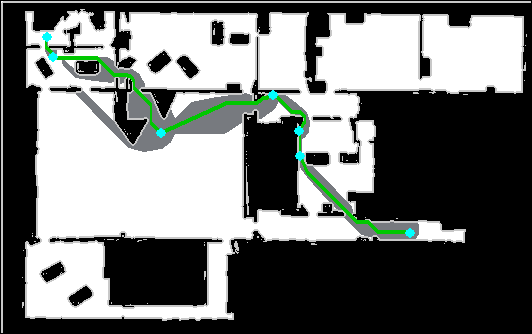
\includegraphics[width=\linewidth]{images/screenshot_137.png}
     \caption{Global Way-point LSTM Planner (max iterations 100)}
  \end{subfigure}
  \hfill
  \begin{subfigure}[b]{0.48\linewidth}
    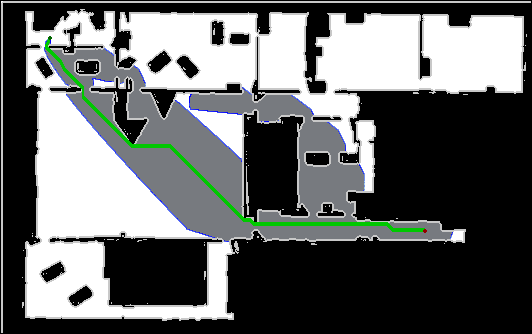
\includegraphics[width=\linewidth]{images/screenshot_109.png}
     \caption{A*\newline}
  \end{subfigure}
  \hfill
  \begin{subfigure}[b]{0.48\linewidth}
    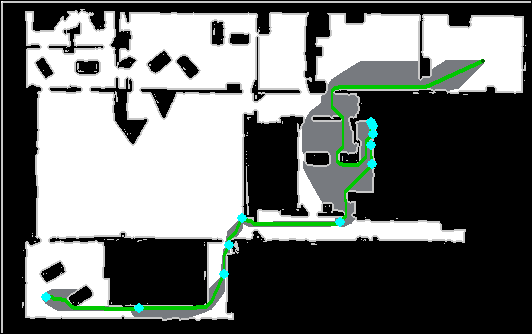
\includegraphics[width=\linewidth]{images/screenshot_138.png}
     \caption{Global Way-point LSTM Planner (max iterations 100)}
  \end{subfigure}
  \hfill
  \begin{subfigure}[b]{0.48\linewidth}
    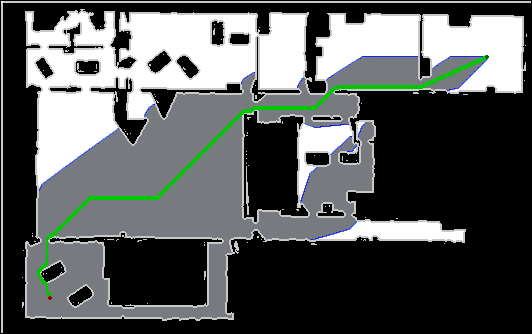
\includegraphics[width=\linewidth]{images/screenshot_110.png}
     \caption{A*\newline}
  \end{subfigure}
  \hfill
  \begin{subfigure}[b]{0.48\linewidth}
    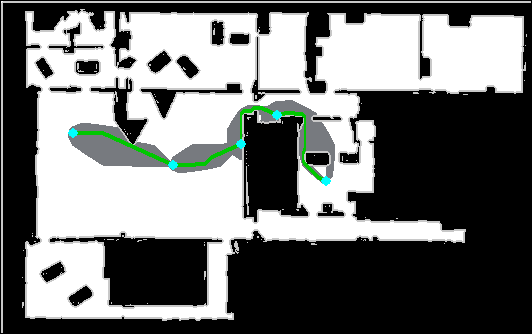
\includegraphics[width=\linewidth]{images/screenshot_140.png}
     \caption{Global Way-point LSTM Planner (max iterations 100)}
  \end{subfigure}
  \hfill
  \begin{subfigure}[b]{0.48\linewidth}
    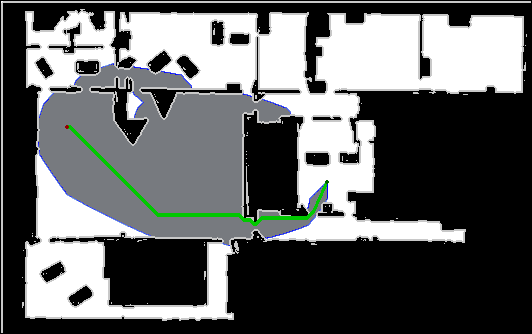
\includegraphics[width=\linewidth]{images/screenshot_114.png}
     \caption{A*\newline}
  \end{subfigure}
  \caption{Global Way-point LSTM Planner vs A* runs on real-world occupancy grid maps \cite{first_map}}
  \label{fig: wp_vs_a_1}
\end{figure}

\begin{figure}[]
  \centering
  \begin{subfigure}[b]{0.38\linewidth}
    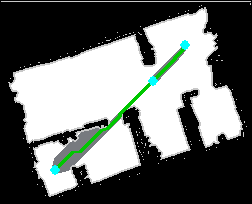
\includegraphics[width=\linewidth]{images/screenshot_141.png}
     \caption{Global Way-point LSTM Planner (max iterations 100)}
  \end{subfigure}
  \hfill
  \begin{subfigure}[b]{0.38\linewidth}
    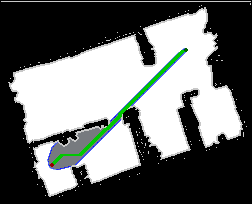
\includegraphics[width=\linewidth]{images/screenshot_116.png}
     \caption{A*\newline}
  \end{subfigure}
  \newline
  \begin{subfigure}[b]{0.38\linewidth}
    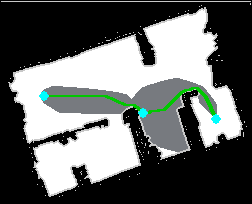
\includegraphics[width=\linewidth]{images/screenshot_142.png}
     \caption{Global Way-point LSTM Planner (max iterations 100)}
  \end{subfigure}
  \hfill
  \begin{subfigure}[b]{0.38\linewidth}
    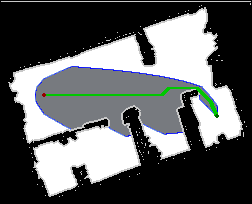
\includegraphics[width=\linewidth]{images/screenshot_117.png}
     \caption{A*\newline}
  \end{subfigure}
  \newline
  \begin{subfigure}[b]{0.38\linewidth}
    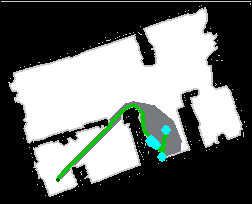
\includegraphics[width=\linewidth]{images/screenshot_143.png}
     \caption{Global Way-point LSTM Planner (max iterations 100)}
  \end{subfigure}
  \hfill
  \begin{subfigure}[b]{0.38\linewidth}
    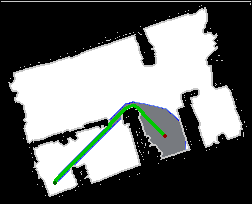
\includegraphics[width=\linewidth]{images/screenshot_118.png}
     \caption{A*\newline}
  \end{subfigure}
  \newline
  \begin{subfigure}[b]{0.38\linewidth}
    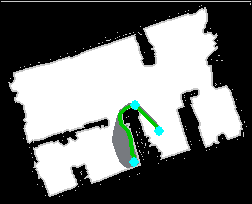
\includegraphics[width=\linewidth]{images/screenshot_147.png}
     \caption{Global Way-point LSTM Planner (max iterations 100)}
  \end{subfigure}
  \hfill
  \begin{subfigure}[b]{0.38\linewidth}
    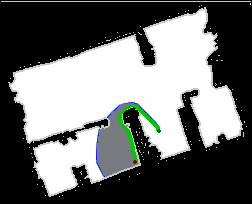
\includegraphics[width=\linewidth]{images/screenshot_146.png}
     \caption{A*\newline}
  \end{subfigure}
  \caption{Global Way-point LSTM Planner vs A* runs on real-world occupancy grid maps \cite{second_map}}
  \label{fig: wp_vs_a_2}
\end{figure}

\begin{figure}[]
  \centering
  \begin{subfigure}[b]{0.40\linewidth}
    
\includegraphics[width=\linewidth]{images/screenshot_144.png}
     \caption{Global Way-point LSTM Planner (max iterations 100)}
  \end{subfigure}
  \hfill
  \begin{subfigure}[b]{0.40\linewidth}
    
\includegraphics[width=\linewidth]{images/screenshot_124.png}
     \caption{A*\newline}
  \end{subfigure}
  \hfill
  \begin{subfigure}[b]{0.40\linewidth}
    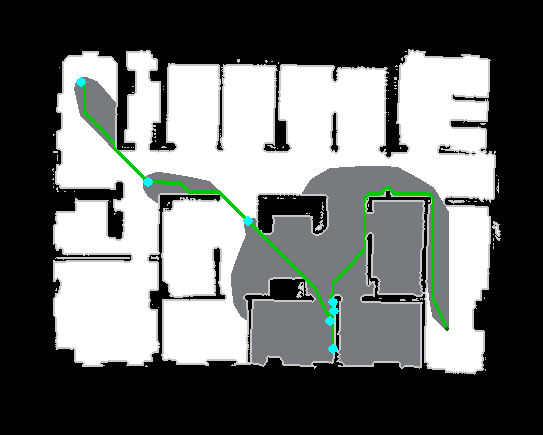
\includegraphics[width=\linewidth]{images/screenshot_148.png}
     \caption{Global Way-point LSTM Planner (max iterations 100)}
  \end{subfigure}
  \hfill
  \begin{subfigure}[b]{0.40\linewidth}
    
\includegraphics[width=\linewidth]{images/screenshot_125.png}
     \caption{A*\newline}
  \end{subfigure}
  \hfill
  \begin{subfigure}[b]{0.40\linewidth}
    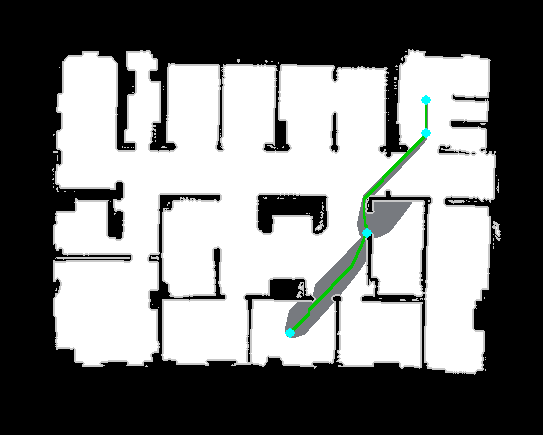
\includegraphics[width=\linewidth]{images/screenshot_149.png}
     \caption{Global Way-point LSTM Planner (max iterations 100)}
  \end{subfigure}
  \hfill
  \begin{subfigure}[b]{0.40\linewidth}
    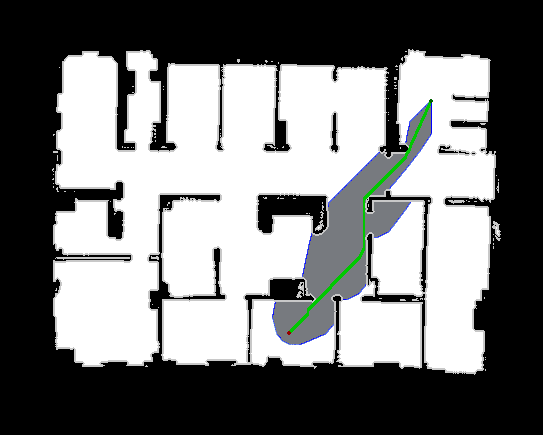
\includegraphics[width=\linewidth]{images/screenshot_126.png}
     \caption{A*\newline}
  \end{subfigure}
  \hfill
  \begin{subfigure}[b]{0.40\linewidth}
    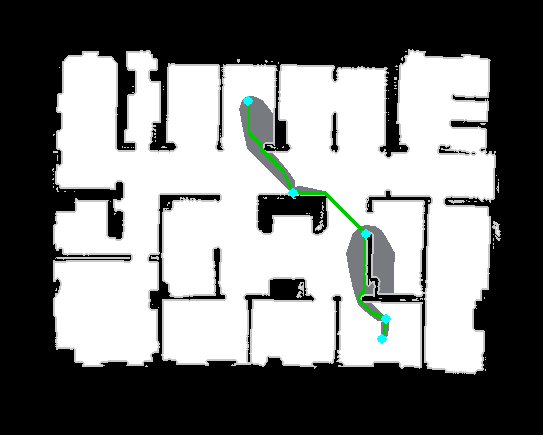
\includegraphics[width=\linewidth]{images/screenshot_150.png}
     \caption{Global Way-point LSTM Planner (max iterations 100)}
  \end{subfigure}
  \hfill
  \begin{subfigure}[b]{0.40\linewidth}
    
\includegraphics[width=\linewidth]{images/screenshot_127.png}
     \caption{A*\newline}
  \end{subfigure}
  \caption{Global Way-point LSTM Planner vs A* runs on real-world occupancy grid maps \cite{third_map}}
  \label{fig: wp_vs_a_3}
\end{figure}

\FloatBarrier

\section{Path Planning on Real-world Robot}
\label{sec: robotexp}

The final evaluation will be run on a real-world robot at Imperial College London (See Figure \ref{fig: robot}). We will use a basic 4-wheeler robot with a YDLidar sensor attached at the top. The YDLidar sensor is a 360-degree two-dimensional distance measurement device which produces a SLAM output image scan \cite{ydlidar}. The robot (Perceptbot) was build as a novel development platform for robotics by a group of students \cite{robo}. The robot has support for multiple hardware attachments (such as an external camera and an Intel Neural Compute Stick for Machine Learning), but we have only used the YDLidar sensor. The motherboard of the robot is a Raspberry Pi circuit board \cite{Halfacree:2012:RPU:2432381} which is running \textit{Raspbian} \cite{raspbian}, and makes use of the \textit{ROS} library for motion controlling.

\begin{figure}[h!]
  \centering
  \begin{subfigure}[b]{0.47\linewidth}
    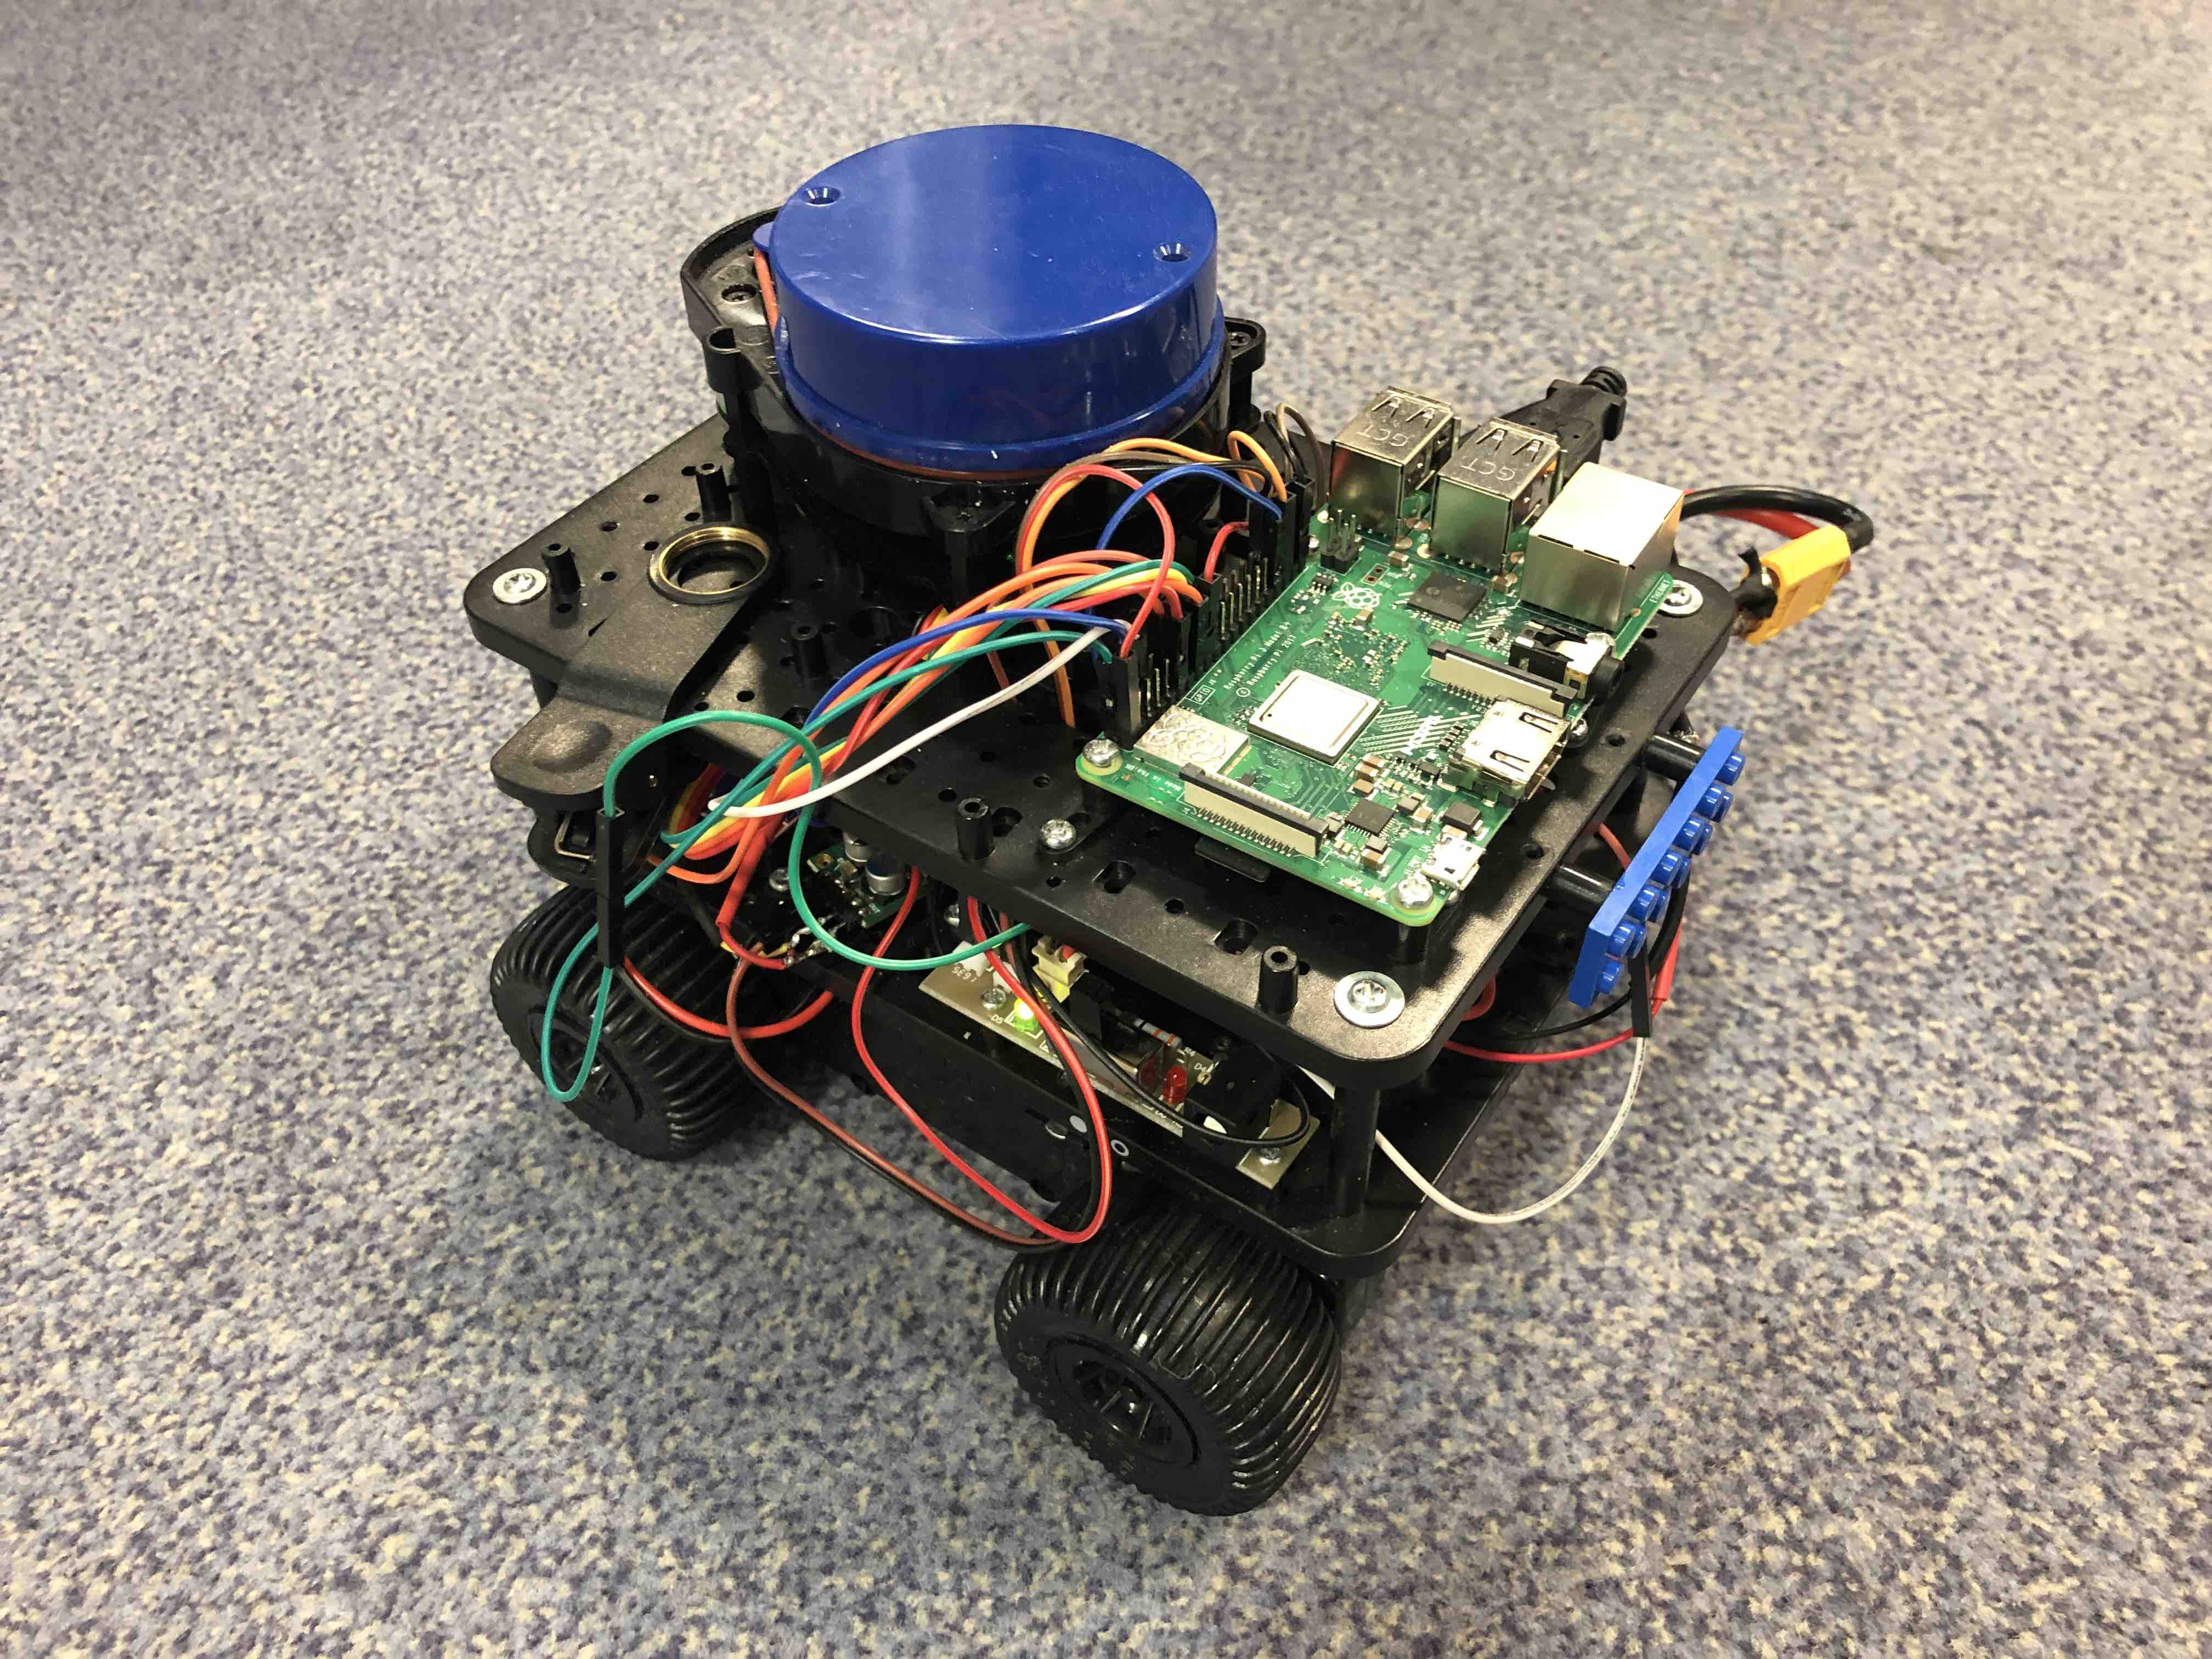
\includegraphics[width=\linewidth]{images/real/robo/preview.JPG}
     \caption{Robot (Perceptbot) with YDLidar Sensor \cite{robo}}
  \end{subfigure}
  \hfill
  \begin{subfigure}[b]{0.47\linewidth}
    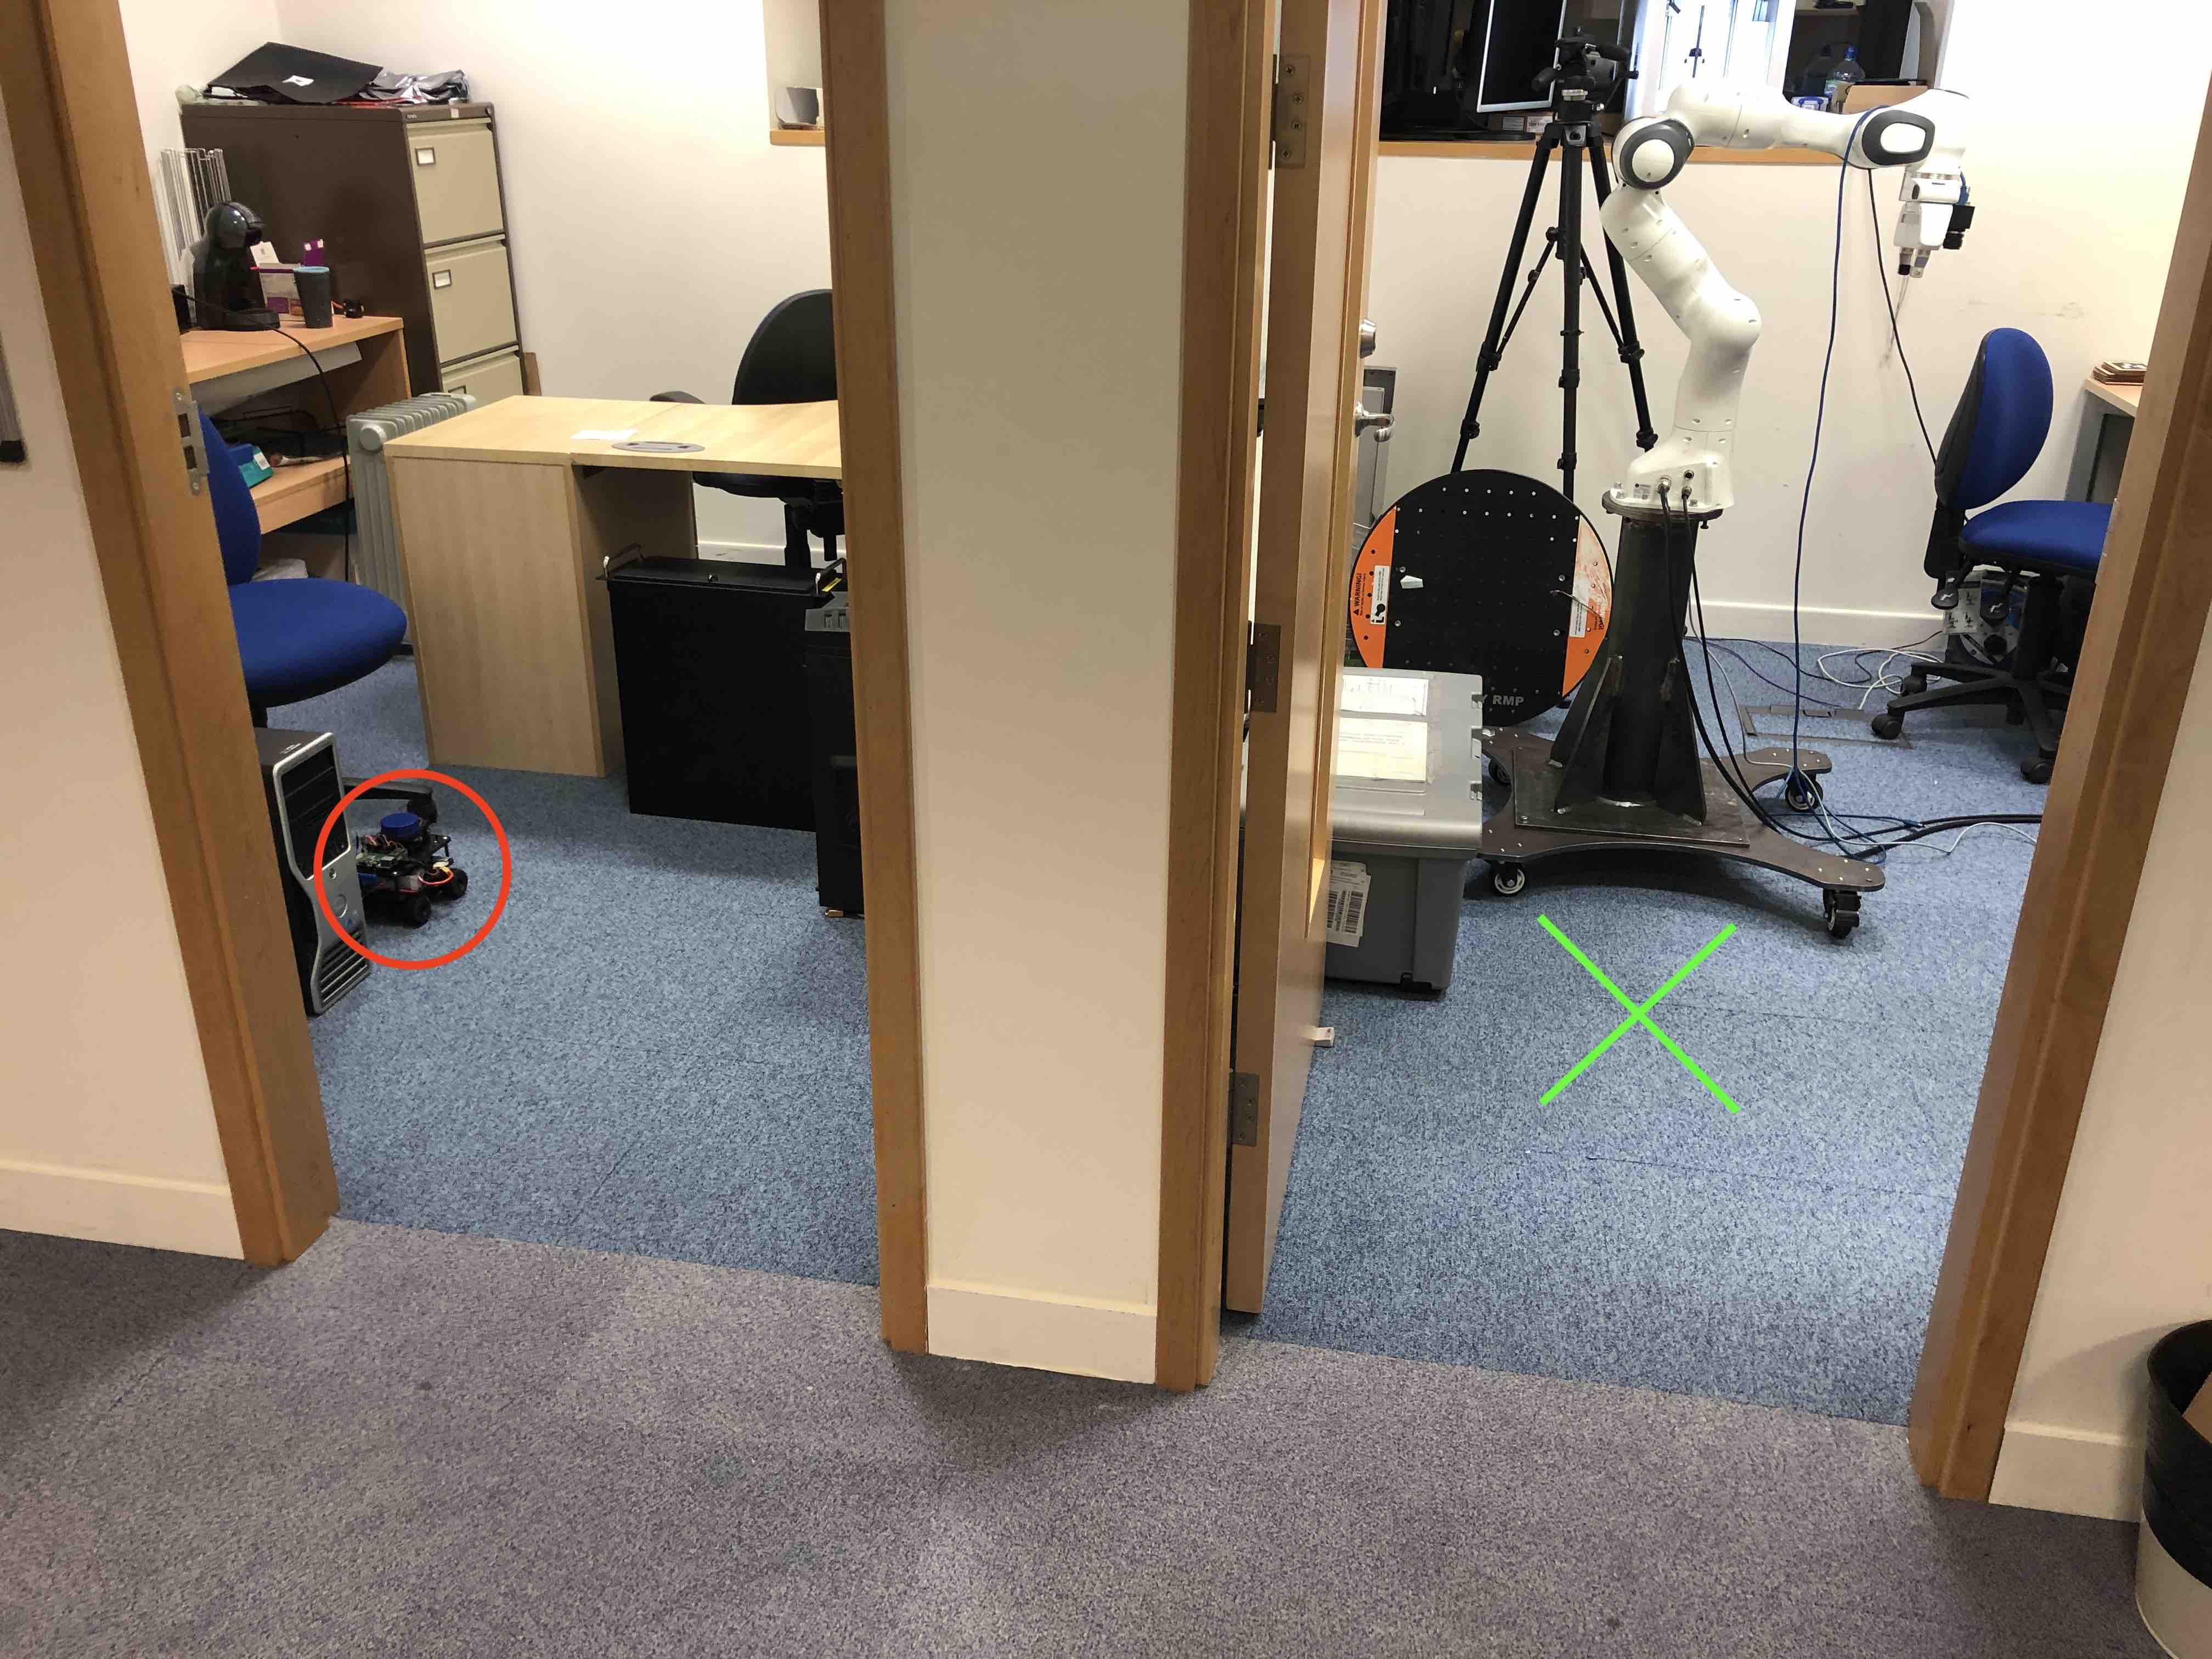
\includegraphics[width=\linewidth]{images/real/robo/start_ann.JPG}
     \caption{Planned trajectory: start and goal positions}
  \end{subfigure}
  \caption{The robot (Perceptbot) (a) and the planned trajectory (b). The red circle represents the robot position (agent) and the green \xmark $\,$ represents the desired destination (goal)}
  \label{fig: robot}
\end{figure}

We have created a \textit{ROS} master node (\textbf{Ros} component) which contains the Global Way-point LSTM Planner and a Motion Planner. The Motion Planner is responsible for physically moving the robot to the specified goal (or way-point), by querying simple velocity control commands using the \textit{cmd\_vel} \textit{ROS} package, and for converting the real world coordinates into PathBench \textbf{Simulator} coordinates and vice-versa. The agent position and rotation is retrieved using the \textit{robot\_pose} \textit{ROS} \textit{package}. The YDLidar sensor is run using the \textit{gmapping} \textit{ROS} package with 0.15 meters grid cell size. Lastly, we have run the \textbf{Ros} master node and \textit{gmapping} on a server which uses network packets (i.e. \textit{ROS} publisher-subscriber APIs) to communicate with the robot. This was done because the performance of the \textit{gmapping} package was severely impacted by the hardware limitations of the Raspberry Pi. The \textbf{Ros} master node could have been run on the Raspberry Pi itself, but we have configured it on the server for faster development and debugging. The \textit{gmapping} SLAM scan output was integrated into PathBench by creating a custom map environment (\textbf{RosMap}), which has support for live updates.

The algorithm starts by converting all trace points generated by the Global Way-point LSTM Planner, including the ones generated by the local kernel, into way-points. The planning between two way-points is achieved by the Motion Planner with simple velocity commands. In the first phase, we rotate the robot so that the robot angle is equal to the angle of the direction to the next way-point. In the second phase, we move in a straight line until we reach the next way-point. If at any point we surpass a pre-defined angle threshold, we correct the robot pose by executing the first phase again, and continue the process. We only request a map update when we have reached the way-points suggested by the global kernel as the local kernel (A*) is offline (See Figure \ref{fig: robot_motion} and Algorithm \ref{alg: real_robot}).

Figure \ref{fig: robot_run} showcases the performance of the real robot on the trajectory defined in Figure \ref{fig: robot}. We will also place the side by side view of the PathBench \textbf{Simulator} and the \textit{ROS} simulator, Rviz. Table \ref{tab: robot_stats} contains the evaluation results reported by our platform.

\pagebreak

\begin{figure}[h!]
  \centering
  \begin{subfigure}[b]{0.4\linewidth}
    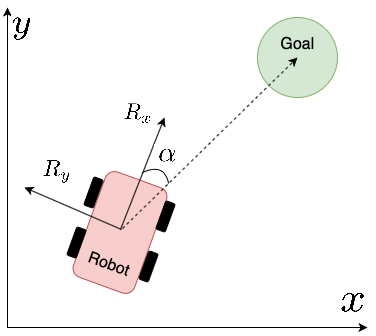
\includegraphics[width=\linewidth]{images/robot.png}
     \caption{First Phase: Rotation}
  \end{subfigure}
  \hfill
  \begin{subfigure}[b]{0.4\linewidth}
    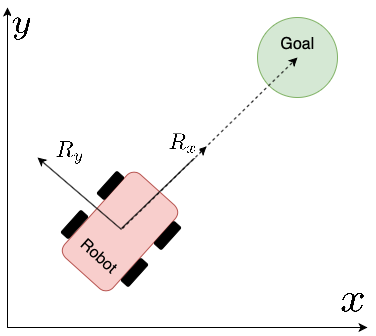
\includegraphics[width=\linewidth]{images/robot_2.png}
     \caption{Second Phase: Forward Movement}
  \end{subfigure}
  \caption{The illustrated two phases of the motion planning between two way-points. $x$ and $y$ are the world coordinate system and $R_x$ and $R_y$ are the robot frame coordinate system}
  \label{fig: robot_motion}
\end{figure}

\begin{algorithm}[h!]
\caption{Robot-Planner}
\label{alg: real_robot}
\begin{algorithmic}[1]

\Procedure{Motion-Planner}{$wp$, $max\_it$, $angle\_threshold$, $goal\_threshold$}
    \For{$i$ in [0, $max\_it$)}
        \State $agent\_pos \gets$ query agent position
        \State $agent\_angle \gets$ query agent angle relative to the world coordinate system
        \State $goal\_dir \gets$ $wp$ - $agent\_pos$
        \State $goal\_angle \gets$ \texttt{arctan2}($goal\_dir.y$, $goal\_dir.x$)
        \State $\alpha \gets$ \texttt{sign}($goal\_angle - agent\_angle$) ($|goal\_angle - agent\_angle|$ \% $\pi$)
        \State
        \If {$\alpha \geq angle\_threshold$}
            \State rotate with velocity proportional to $\alpha$
            \State \textbf{continue}
        \EndIf
        \State
        \If {$\norm{goal\_dir}_{2} \geq dist\_threshold$}
            \State move forward with velocity proportional to $\norm{goal\_dir}_{2}$
            \State \textbf{continue}
        \Else
            \State \textbf{return}
        \EndIf
    \EndFor
    \State
\EndProcedure

\Procedure{Robot-Planner}{$M\colon(A, Os, G)$}
    \While {goal is not reached}
        \State $M \gets$ query new SLAM scan
        \State $way\_points \gets$ get Global Way-point LSTM Planner trace until next global way-point
        \State
        \For {$wp$ in $way\_points$}
            \State \textit{Motion-Planner}($wp$, 1000, 0.1, 0.1)
        \EndFor
        \State
        \If {there are no $way\_points$}
            \State goal was not found
            \State \textbf{break}
        \EndIf
    \EndWhile
\EndProcedure
\end{algorithmic}
\end{algorithm}

\pagebreak

\begin{figure}[h!]
  \centering
  \begin{subfigure}[b]{0.32\linewidth}
    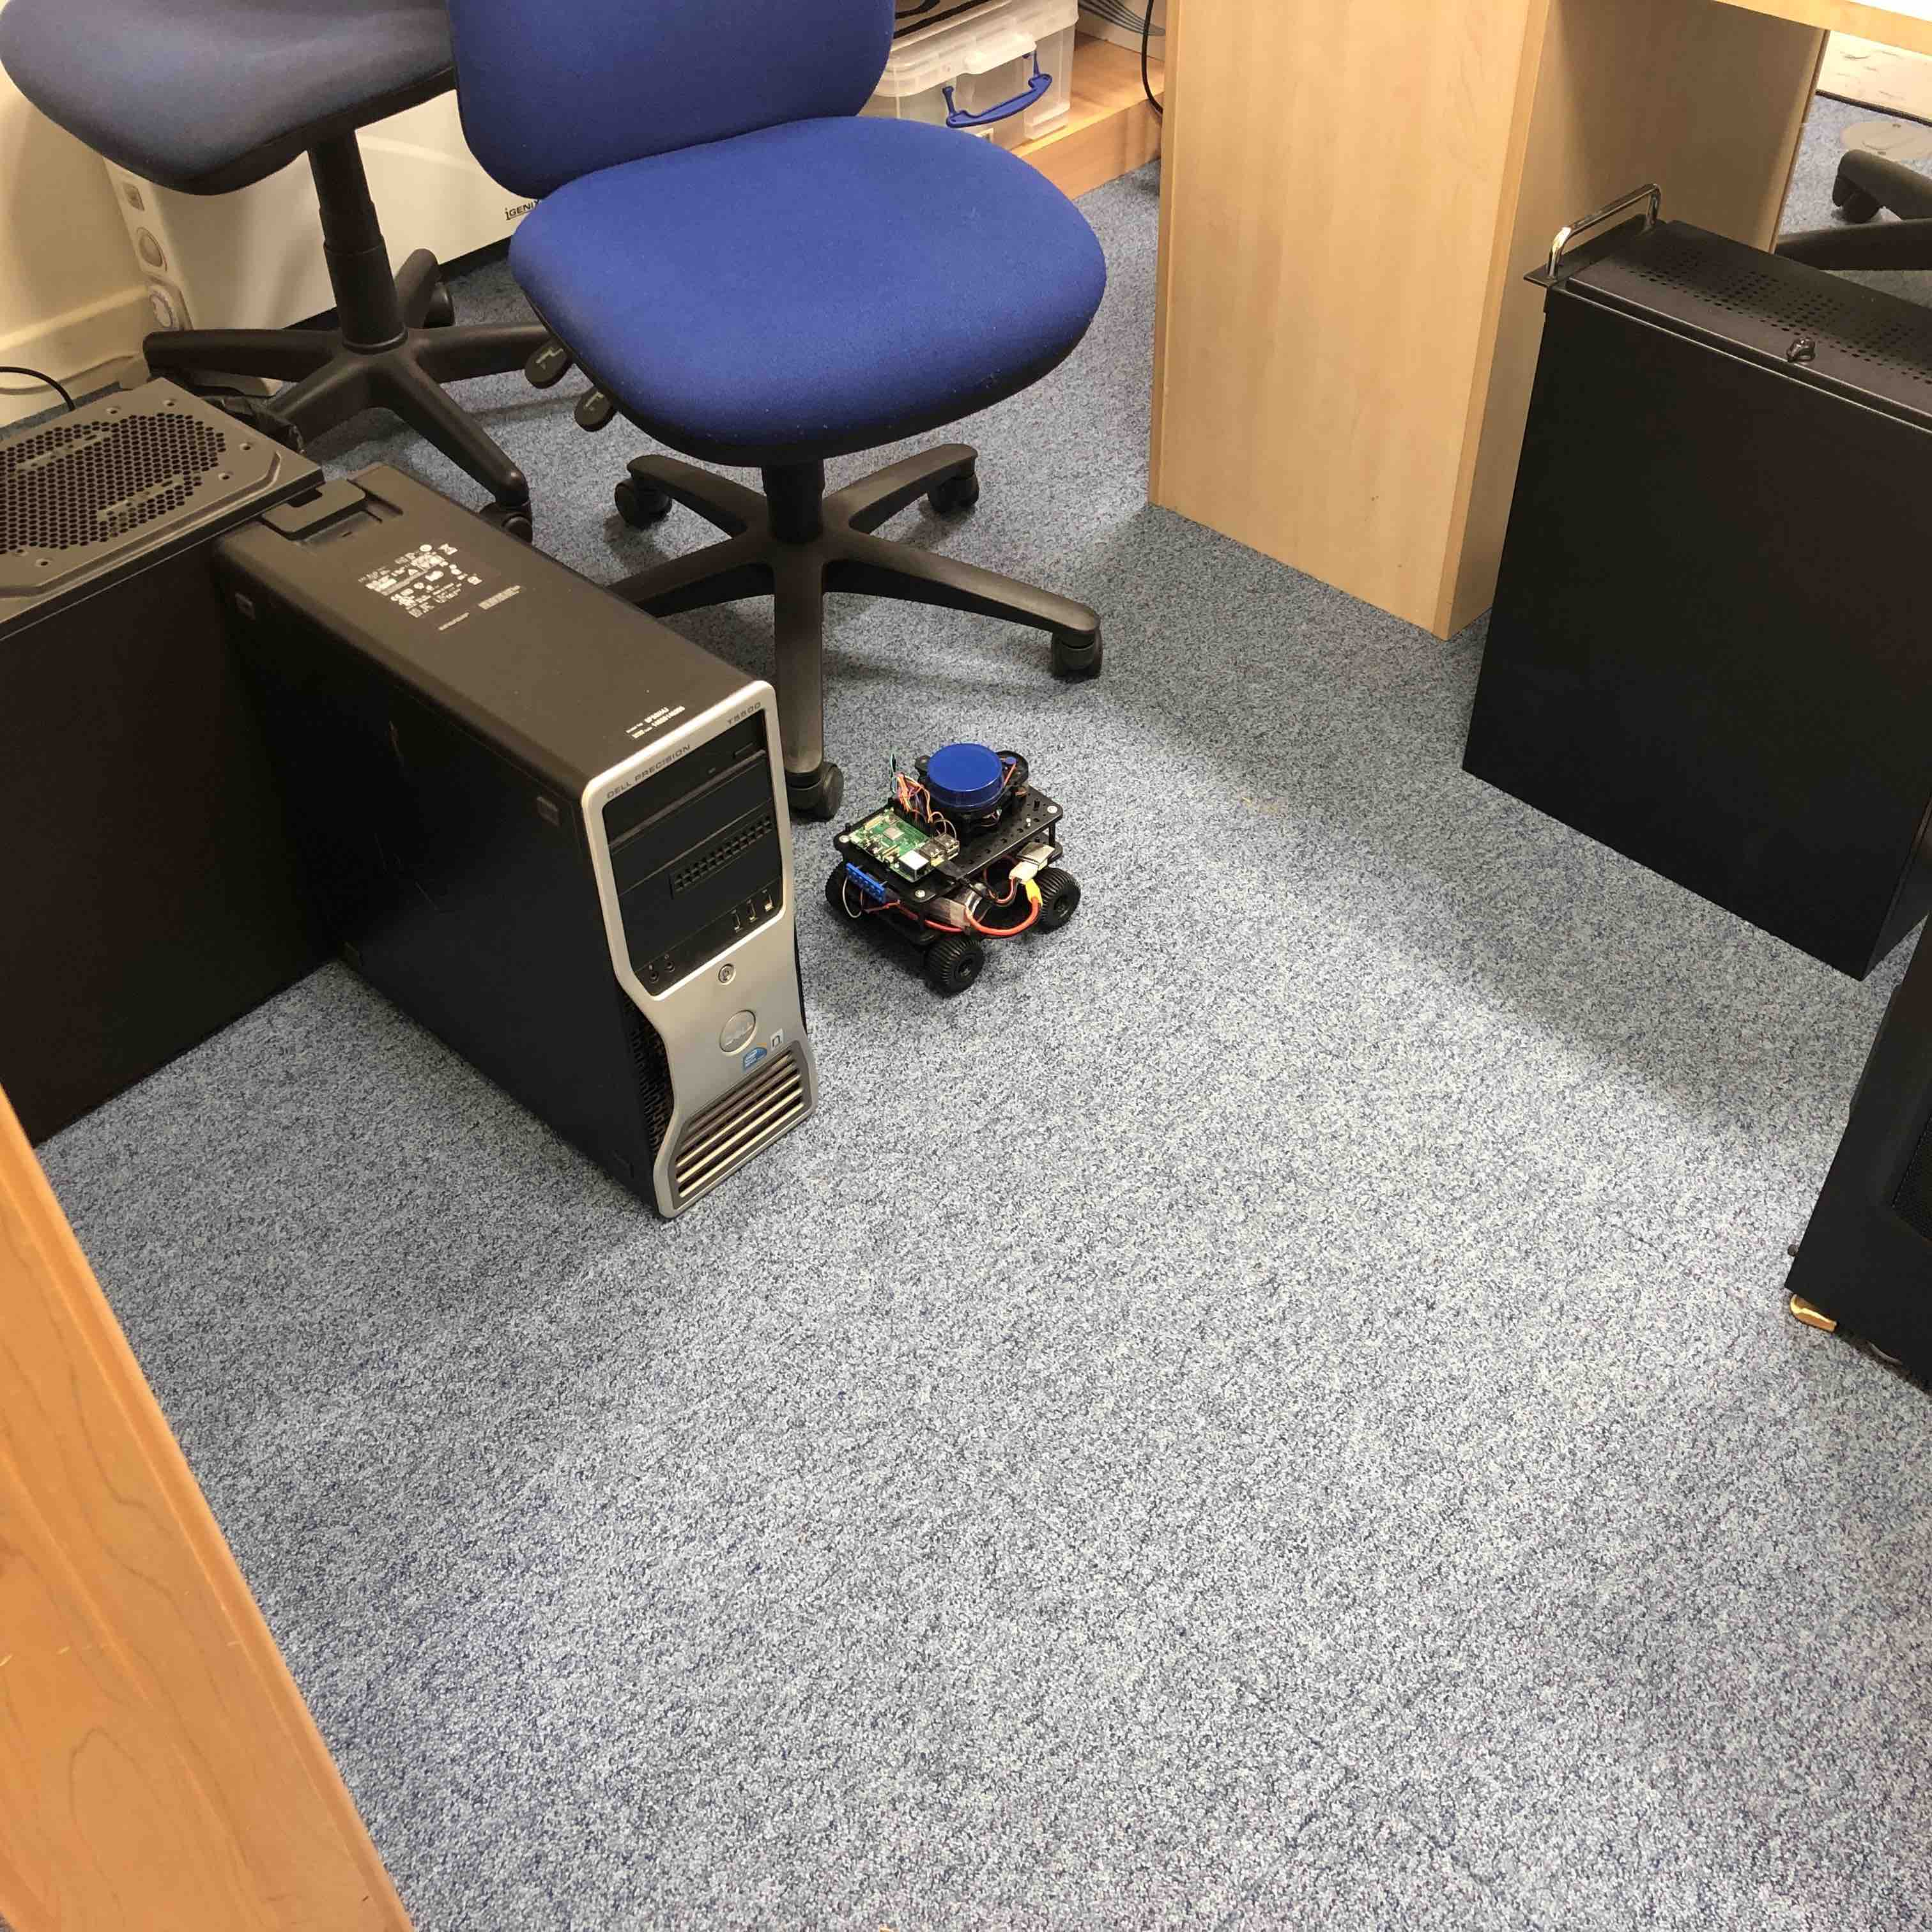
\includegraphics[width=\linewidth]{images/real/robo/start_2.JPG}
     \caption{Real-world: Start}
  \end{subfigure}
  \hfill
  \begin{subfigure}[b]{0.32\linewidth}
    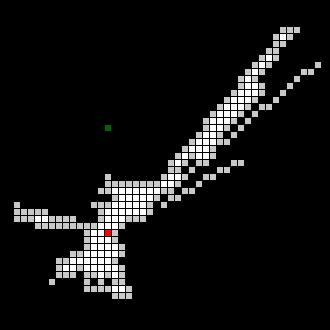
\includegraphics[width=\linewidth]{images/real/sys/start_2.png}
     \caption{PathBench: Start}
  \end{subfigure}
  \hfill
  \begin{subfigure}[b]{0.32\linewidth}
    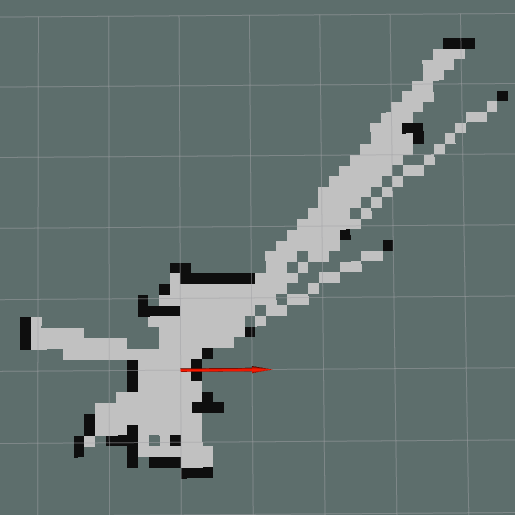
\includegraphics[width=\linewidth]{images/real/sys/start_3.png}
     \caption{Rviz: Start}
  \end{subfigure}
  
  \newline
  
  \begin{subfigure}[b]{0.32\linewidth}
    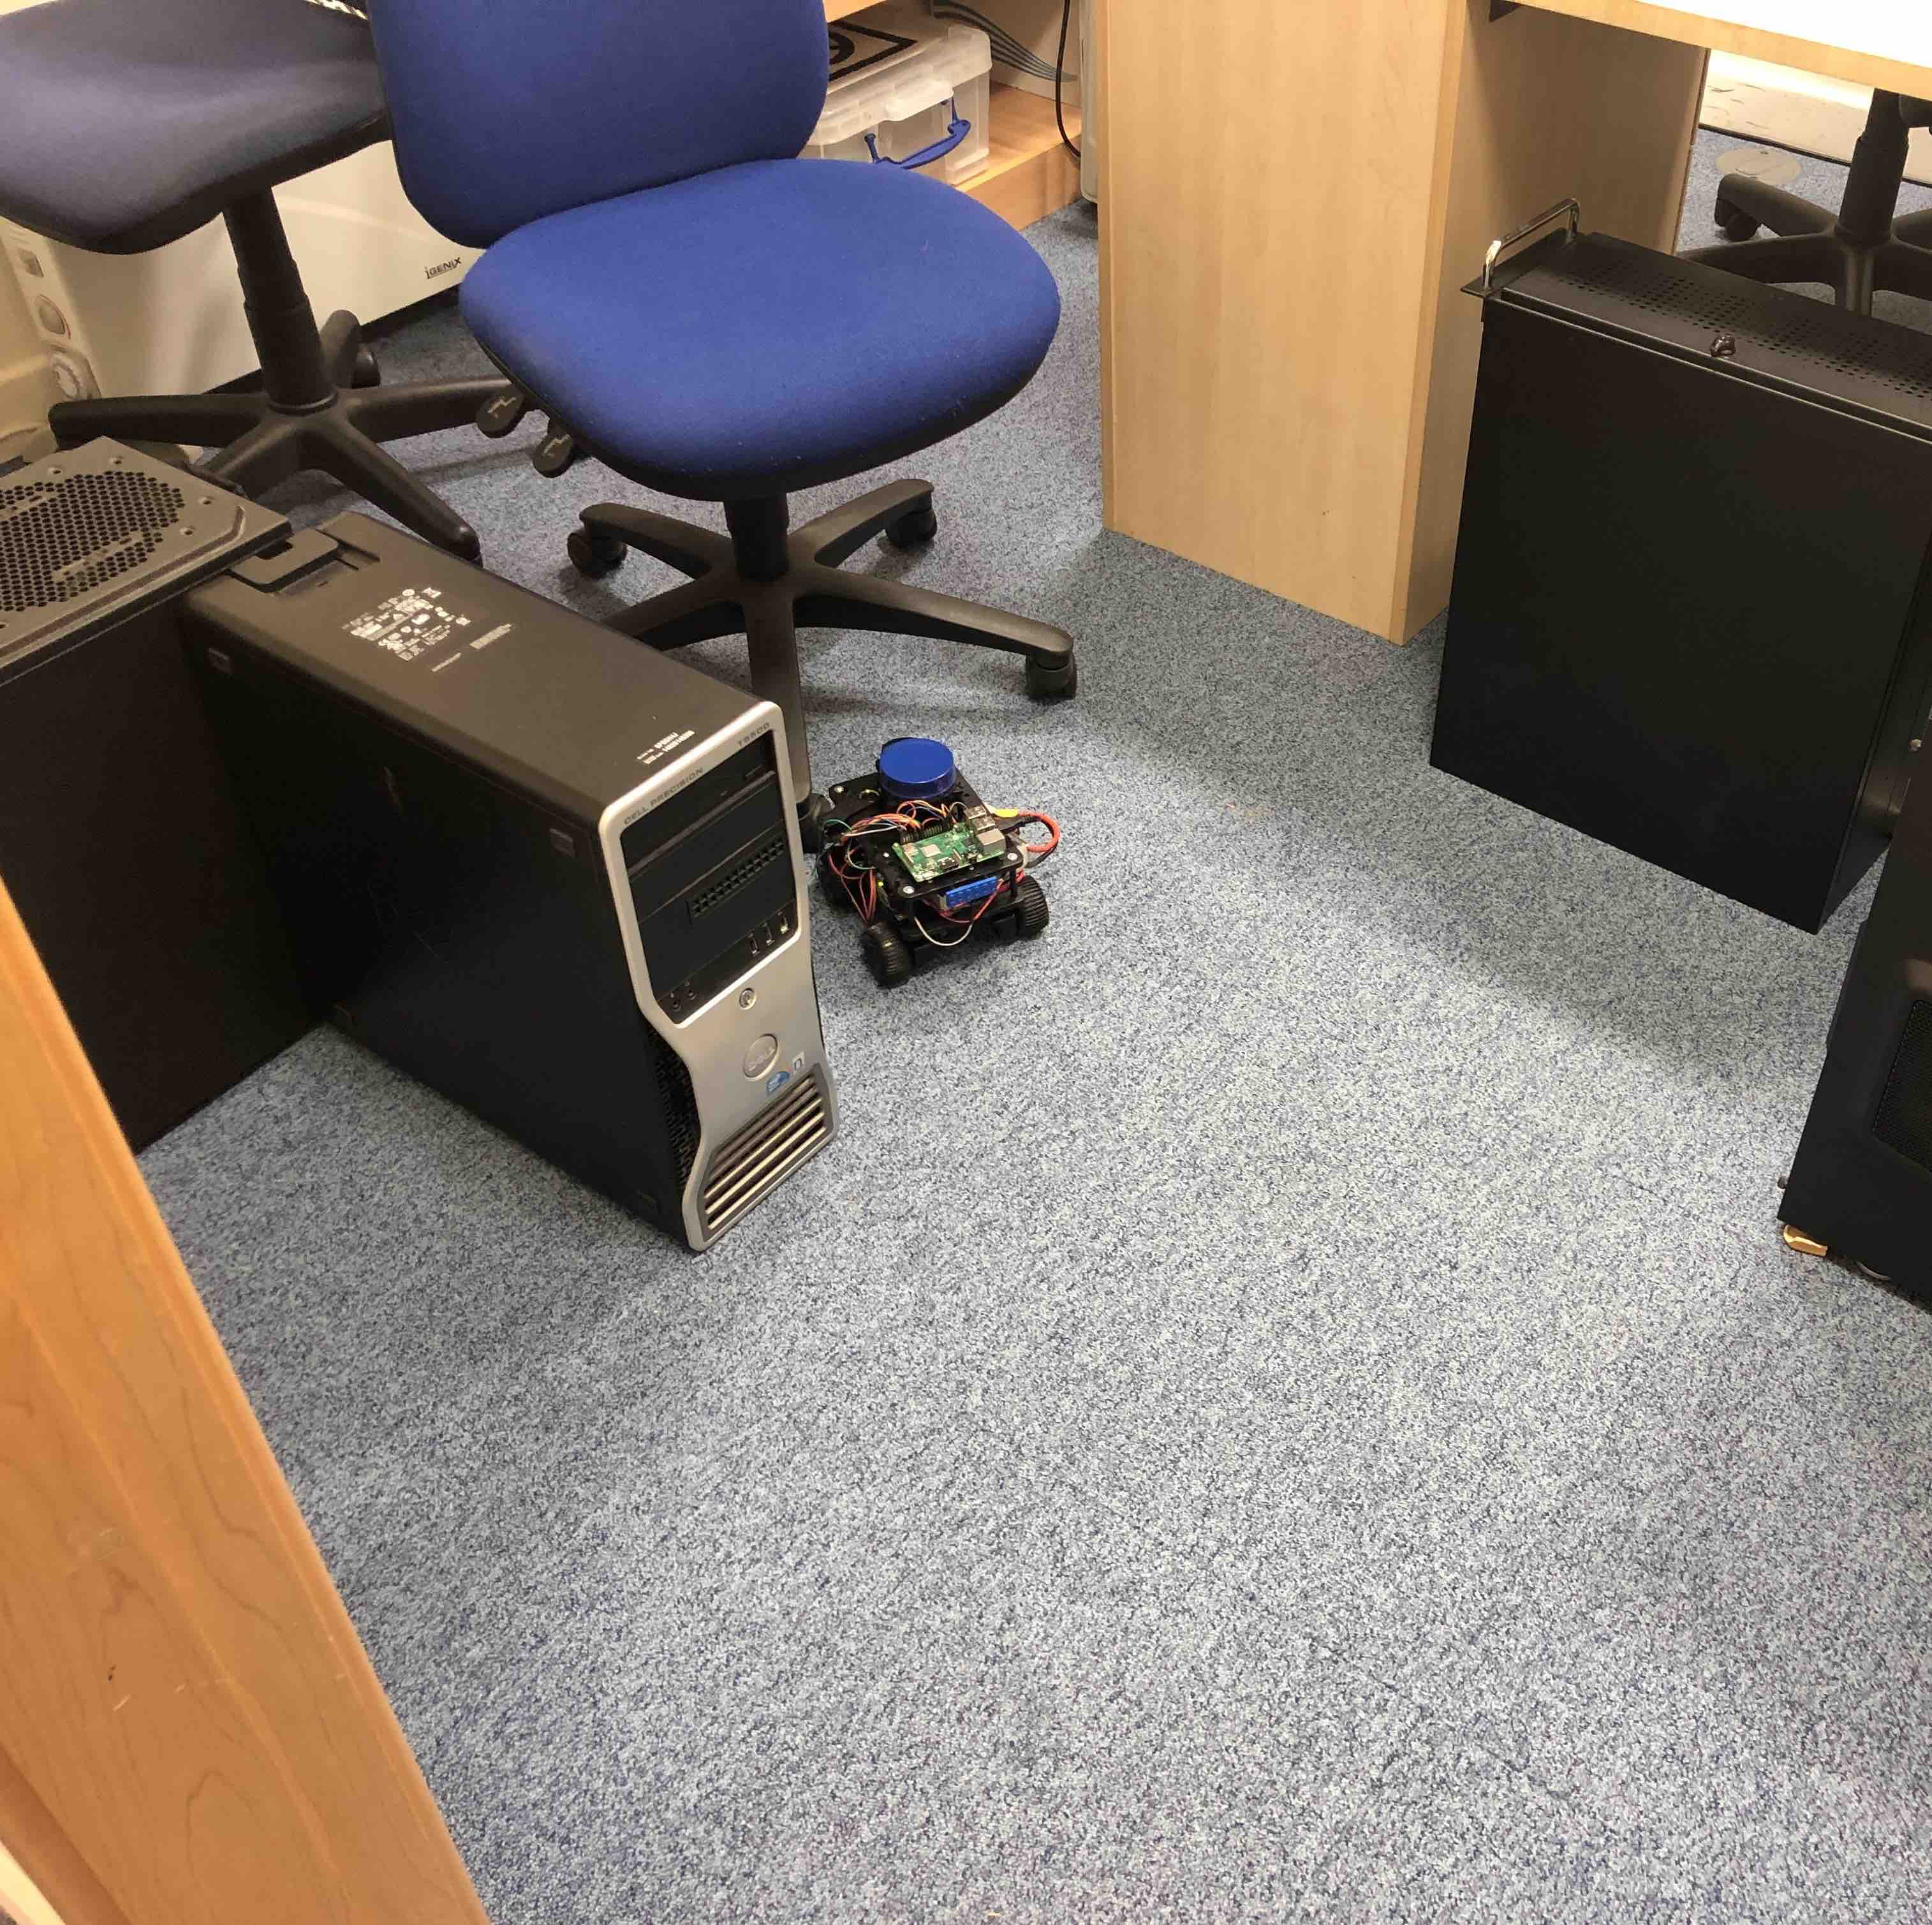
\includegraphics[width=\linewidth]{images/real/robo/1.JPG}
     \caption{Real-world: Suggested WP 1}
  \end{subfigure}
  \hfill
  \begin{subfigure}[b]{0.32\linewidth}
    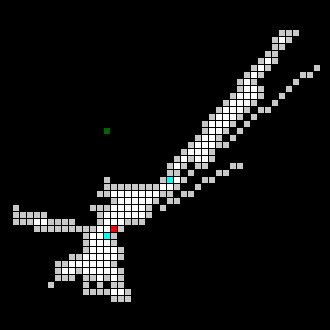
\includegraphics[width=\linewidth]{images/real/sys/1_2.png}
     \caption{PathBench: Suggested WP 1}
  \end{subfigure}
  \hfill
  \begin{subfigure}[b]{0.32\linewidth}
    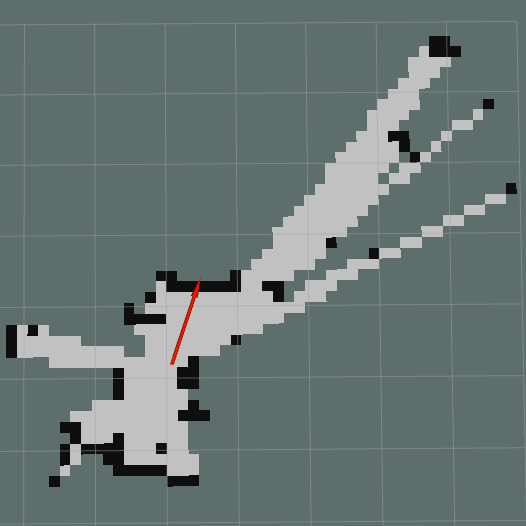
\includegraphics[width=\linewidth]{images/real/sys/1_3.png}
     \caption{Rviz: Suggested WP 1}
  \end{subfigure}
  
  \newline
  
  \begin{subfigure}[b]{0.32\linewidth}
    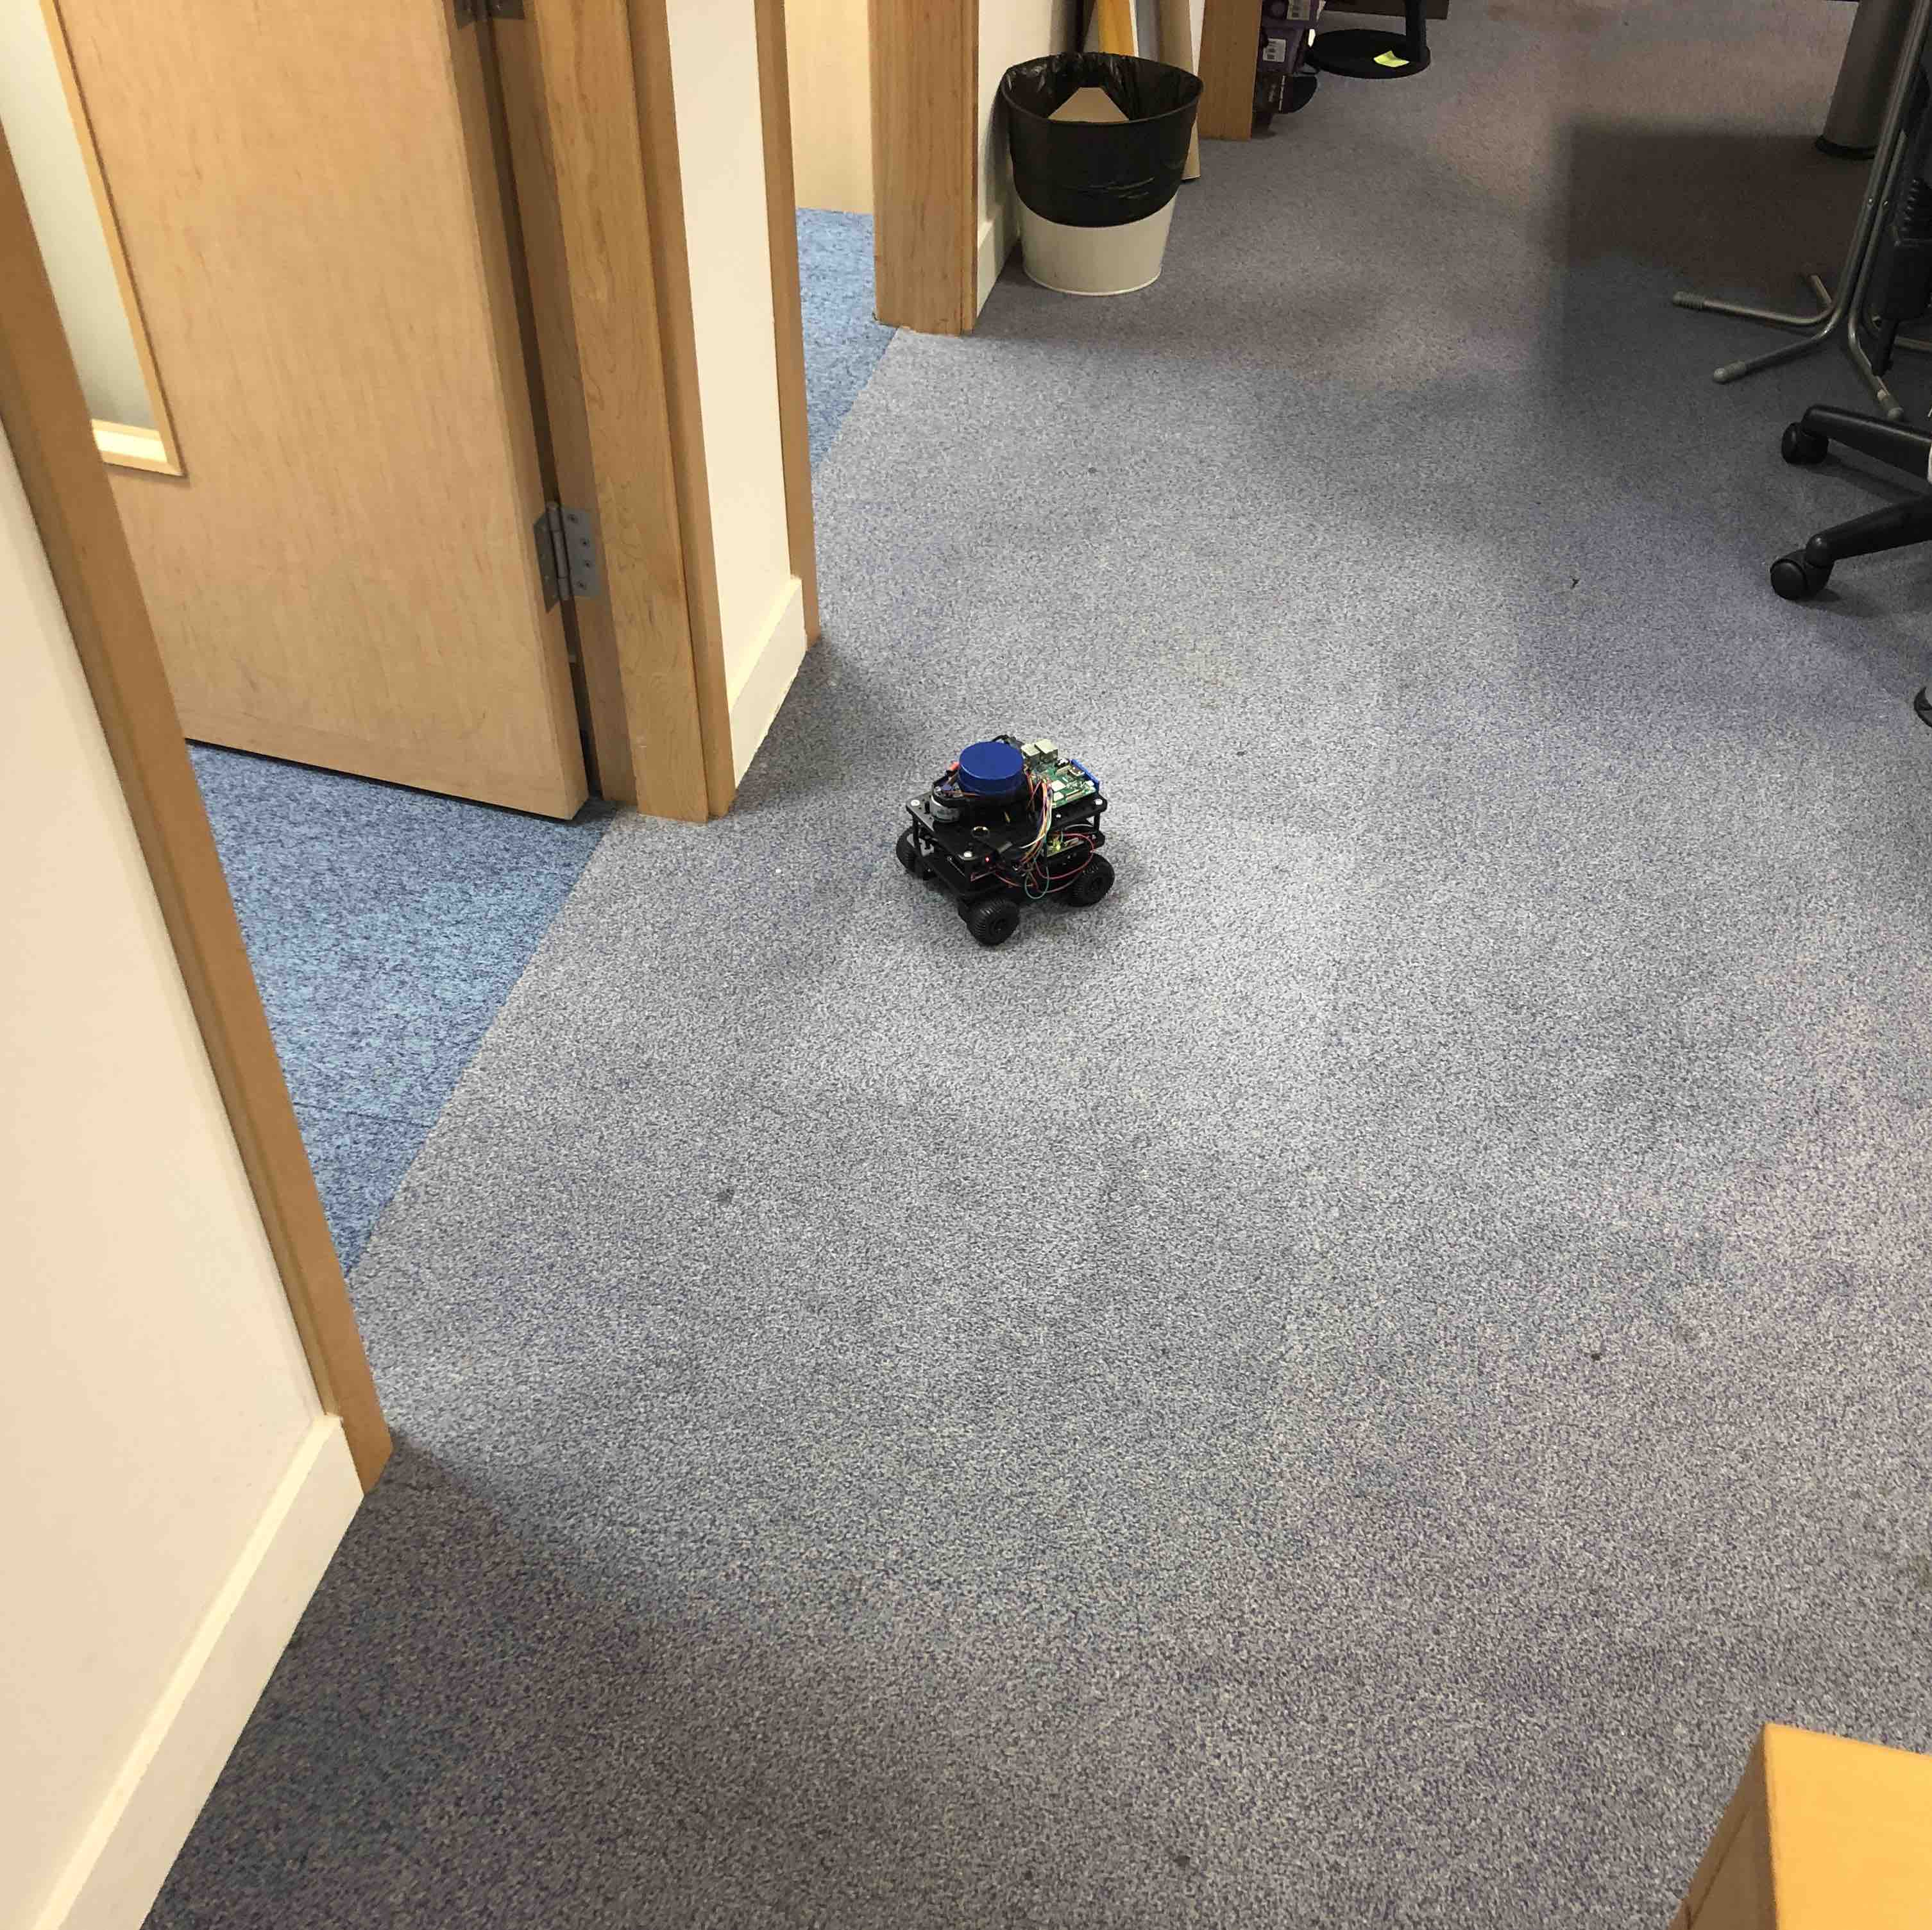
\includegraphics[width=\linewidth]{images/real/robo/2.JPG}
     \caption{Real-world: Reached WP 1}
  \end{subfigure}
  \hfill
  \begin{subfigure}[b]{0.32\linewidth}
    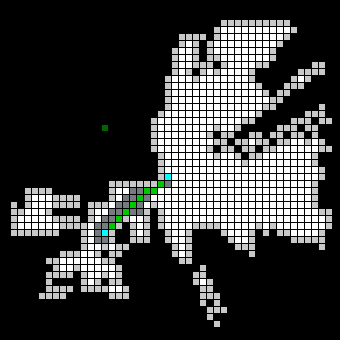
\includegraphics[width=\linewidth]{images/real/sys/2_2.png}
     \caption{PathBench: Reached WP 1}
  \end{subfigure}
  \hfill
  \begin{subfigure}[b]{0.32\linewidth}
    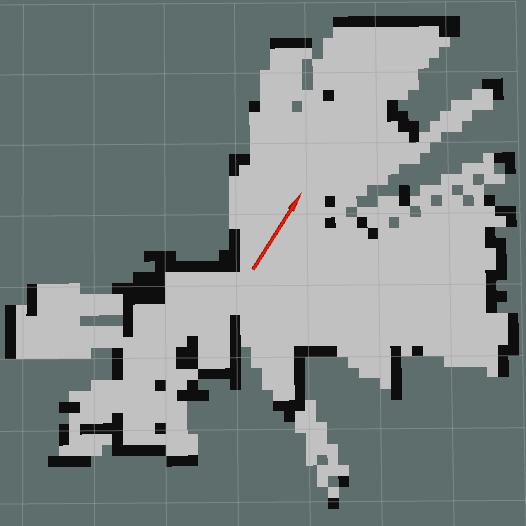
\includegraphics[width=\linewidth]{images/real/sys/2_3.png}
     \caption{Rviz: Reached WP 1}
  \end{subfigure}
  
  \newline
  
  \begin{subfigure}[b]{0.32\linewidth}
    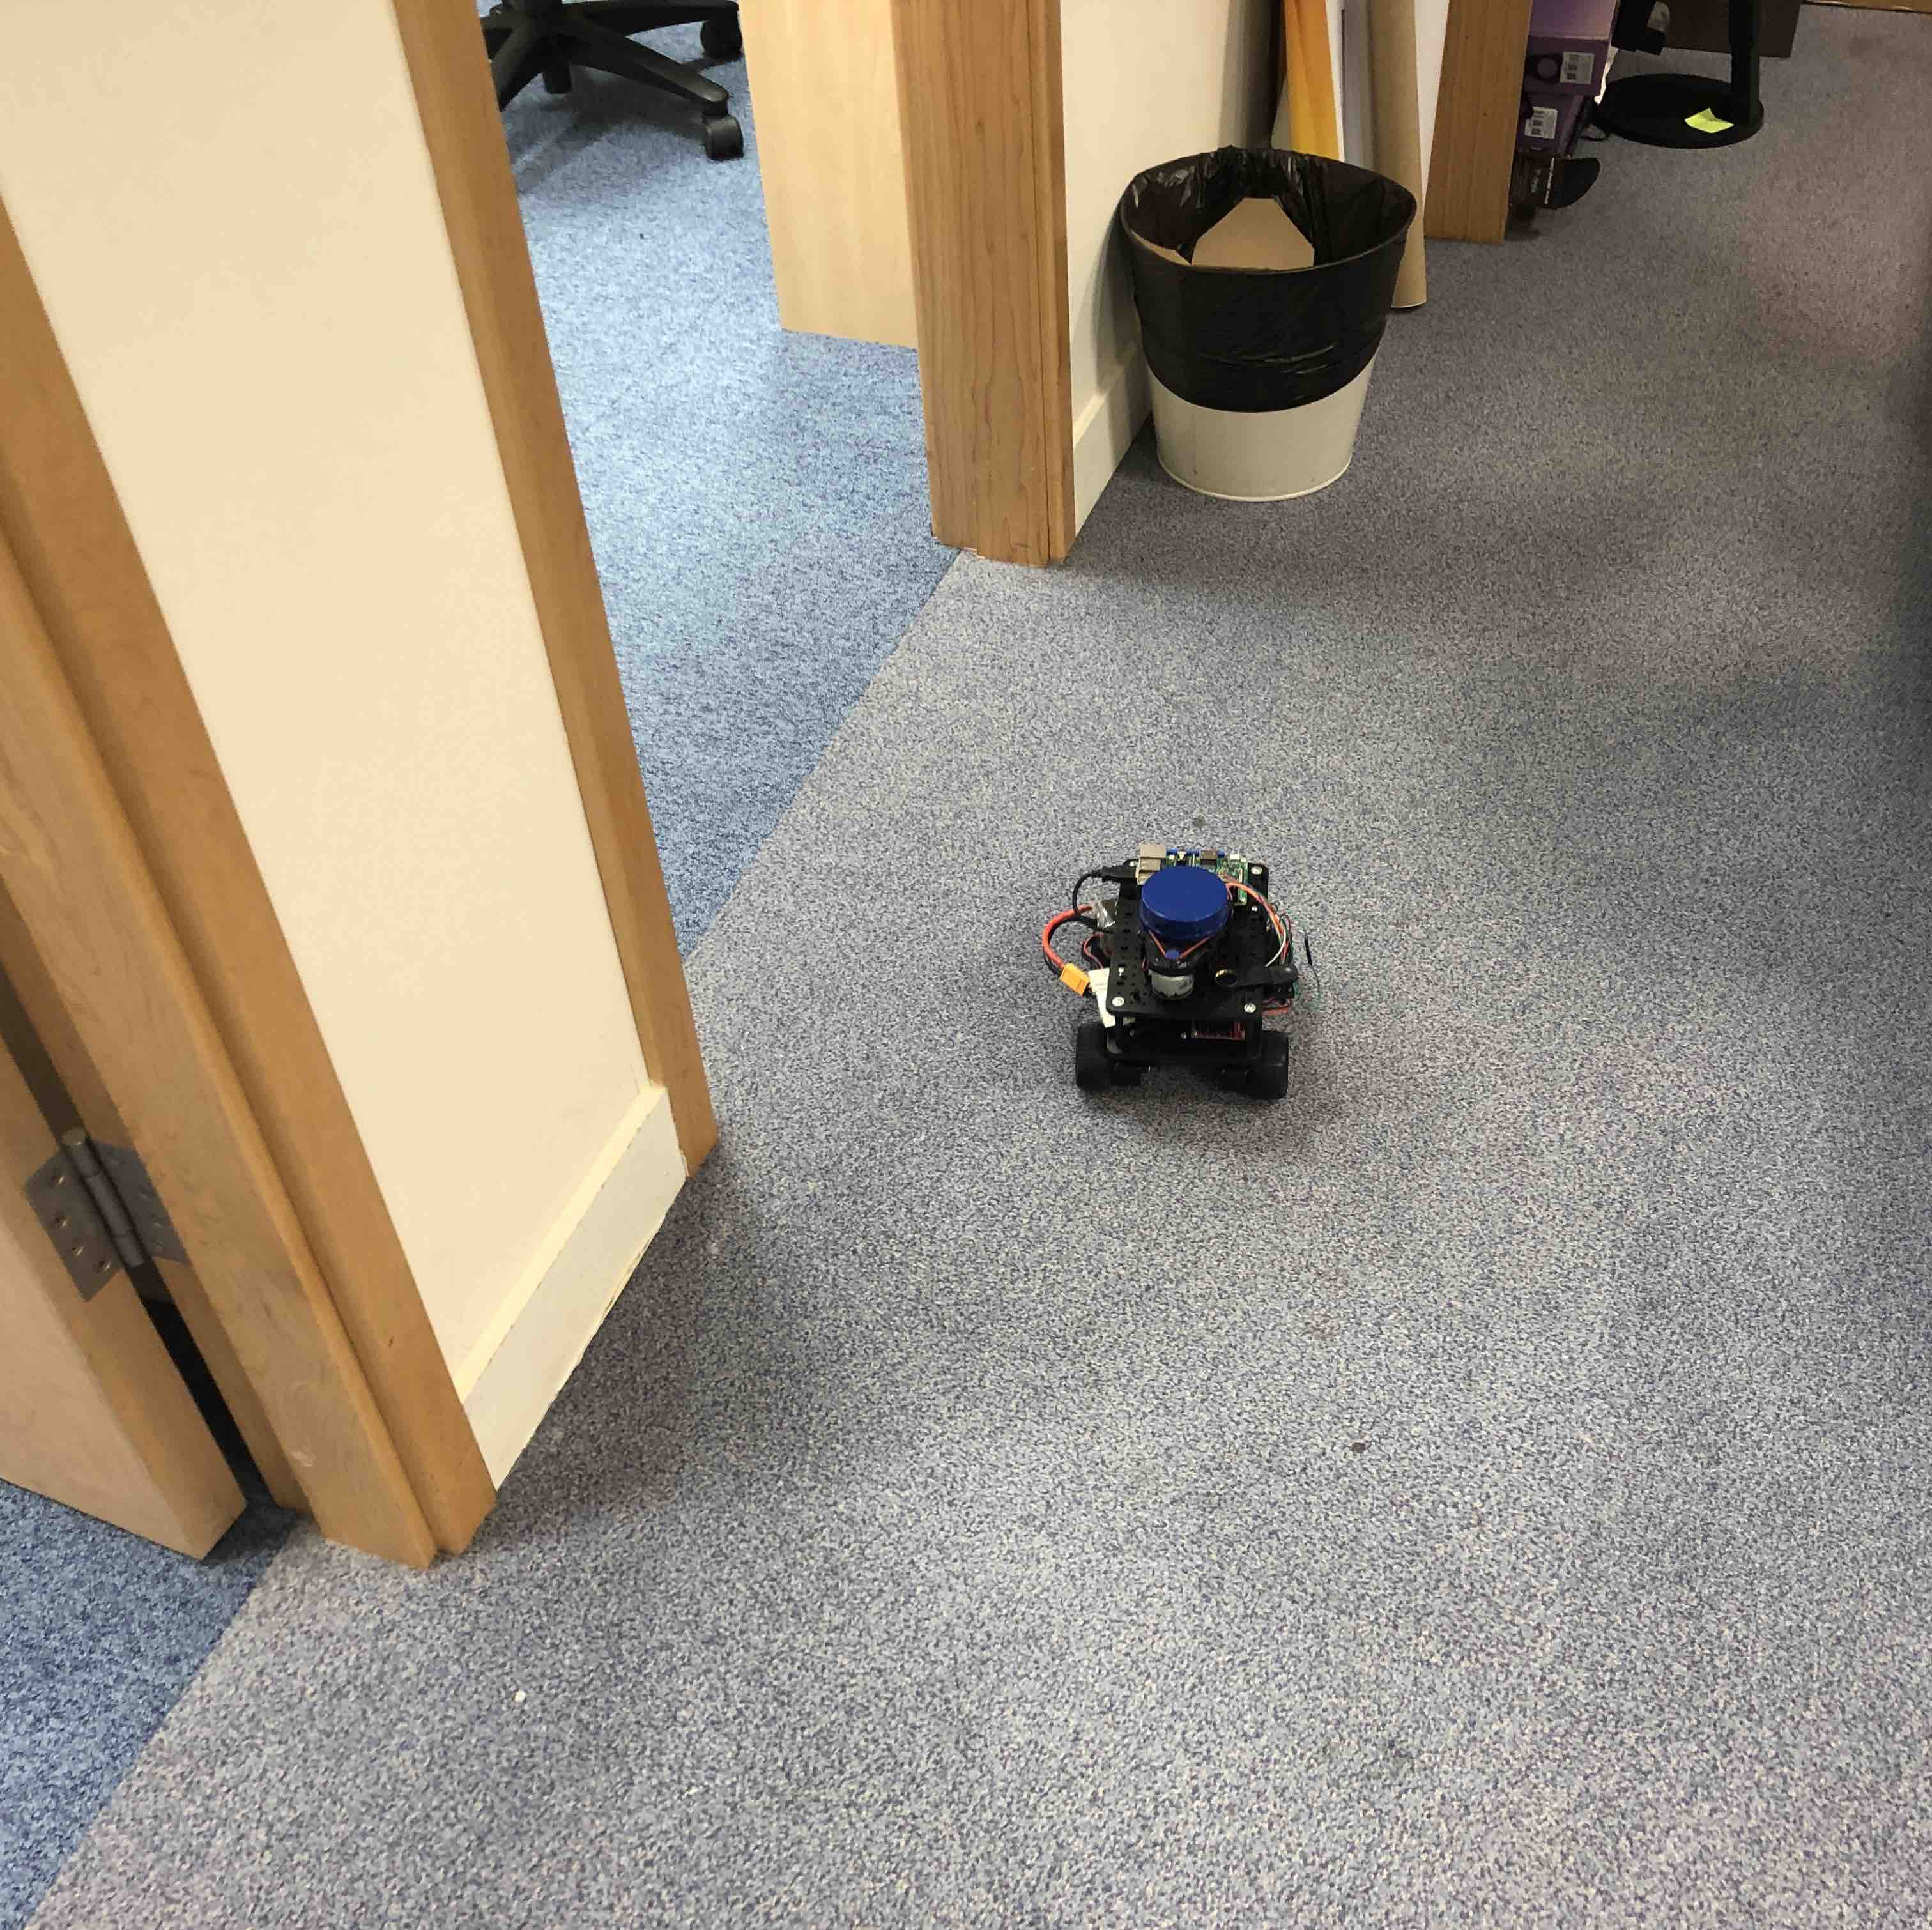
\includegraphics[width=\linewidth]{images/real/robo/3.JPG}
     \caption{Real-world: Suggested WP 2}
  \end{subfigure}
  \hfill
  \begin{subfigure}[b]{0.32\linewidth}
    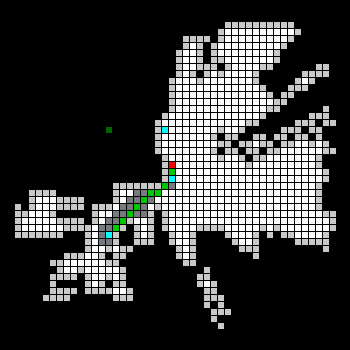
\includegraphics[width=\linewidth]{images/real/sys/3_2.png}
     \caption{PathBench: Suggested WP 2}
  \end{subfigure}
  \hfill
  \begin{subfigure}[b]{0.32\linewidth}
    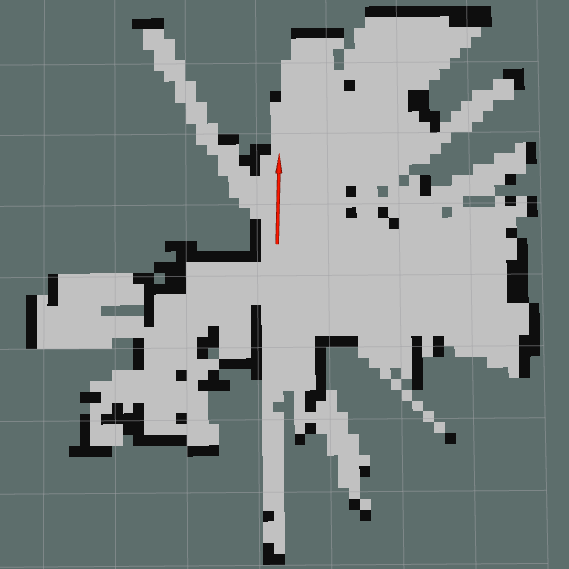
\includegraphics[width=\linewidth]{images/real/sys/3_3.png}
     \caption{Rviz: Suggested WP 2}
  \end{subfigure}
\end{figure}

\begin{figure}[htb]\ContinuedFloat
  \begin{subfigure}[b]{0.32\linewidth}
    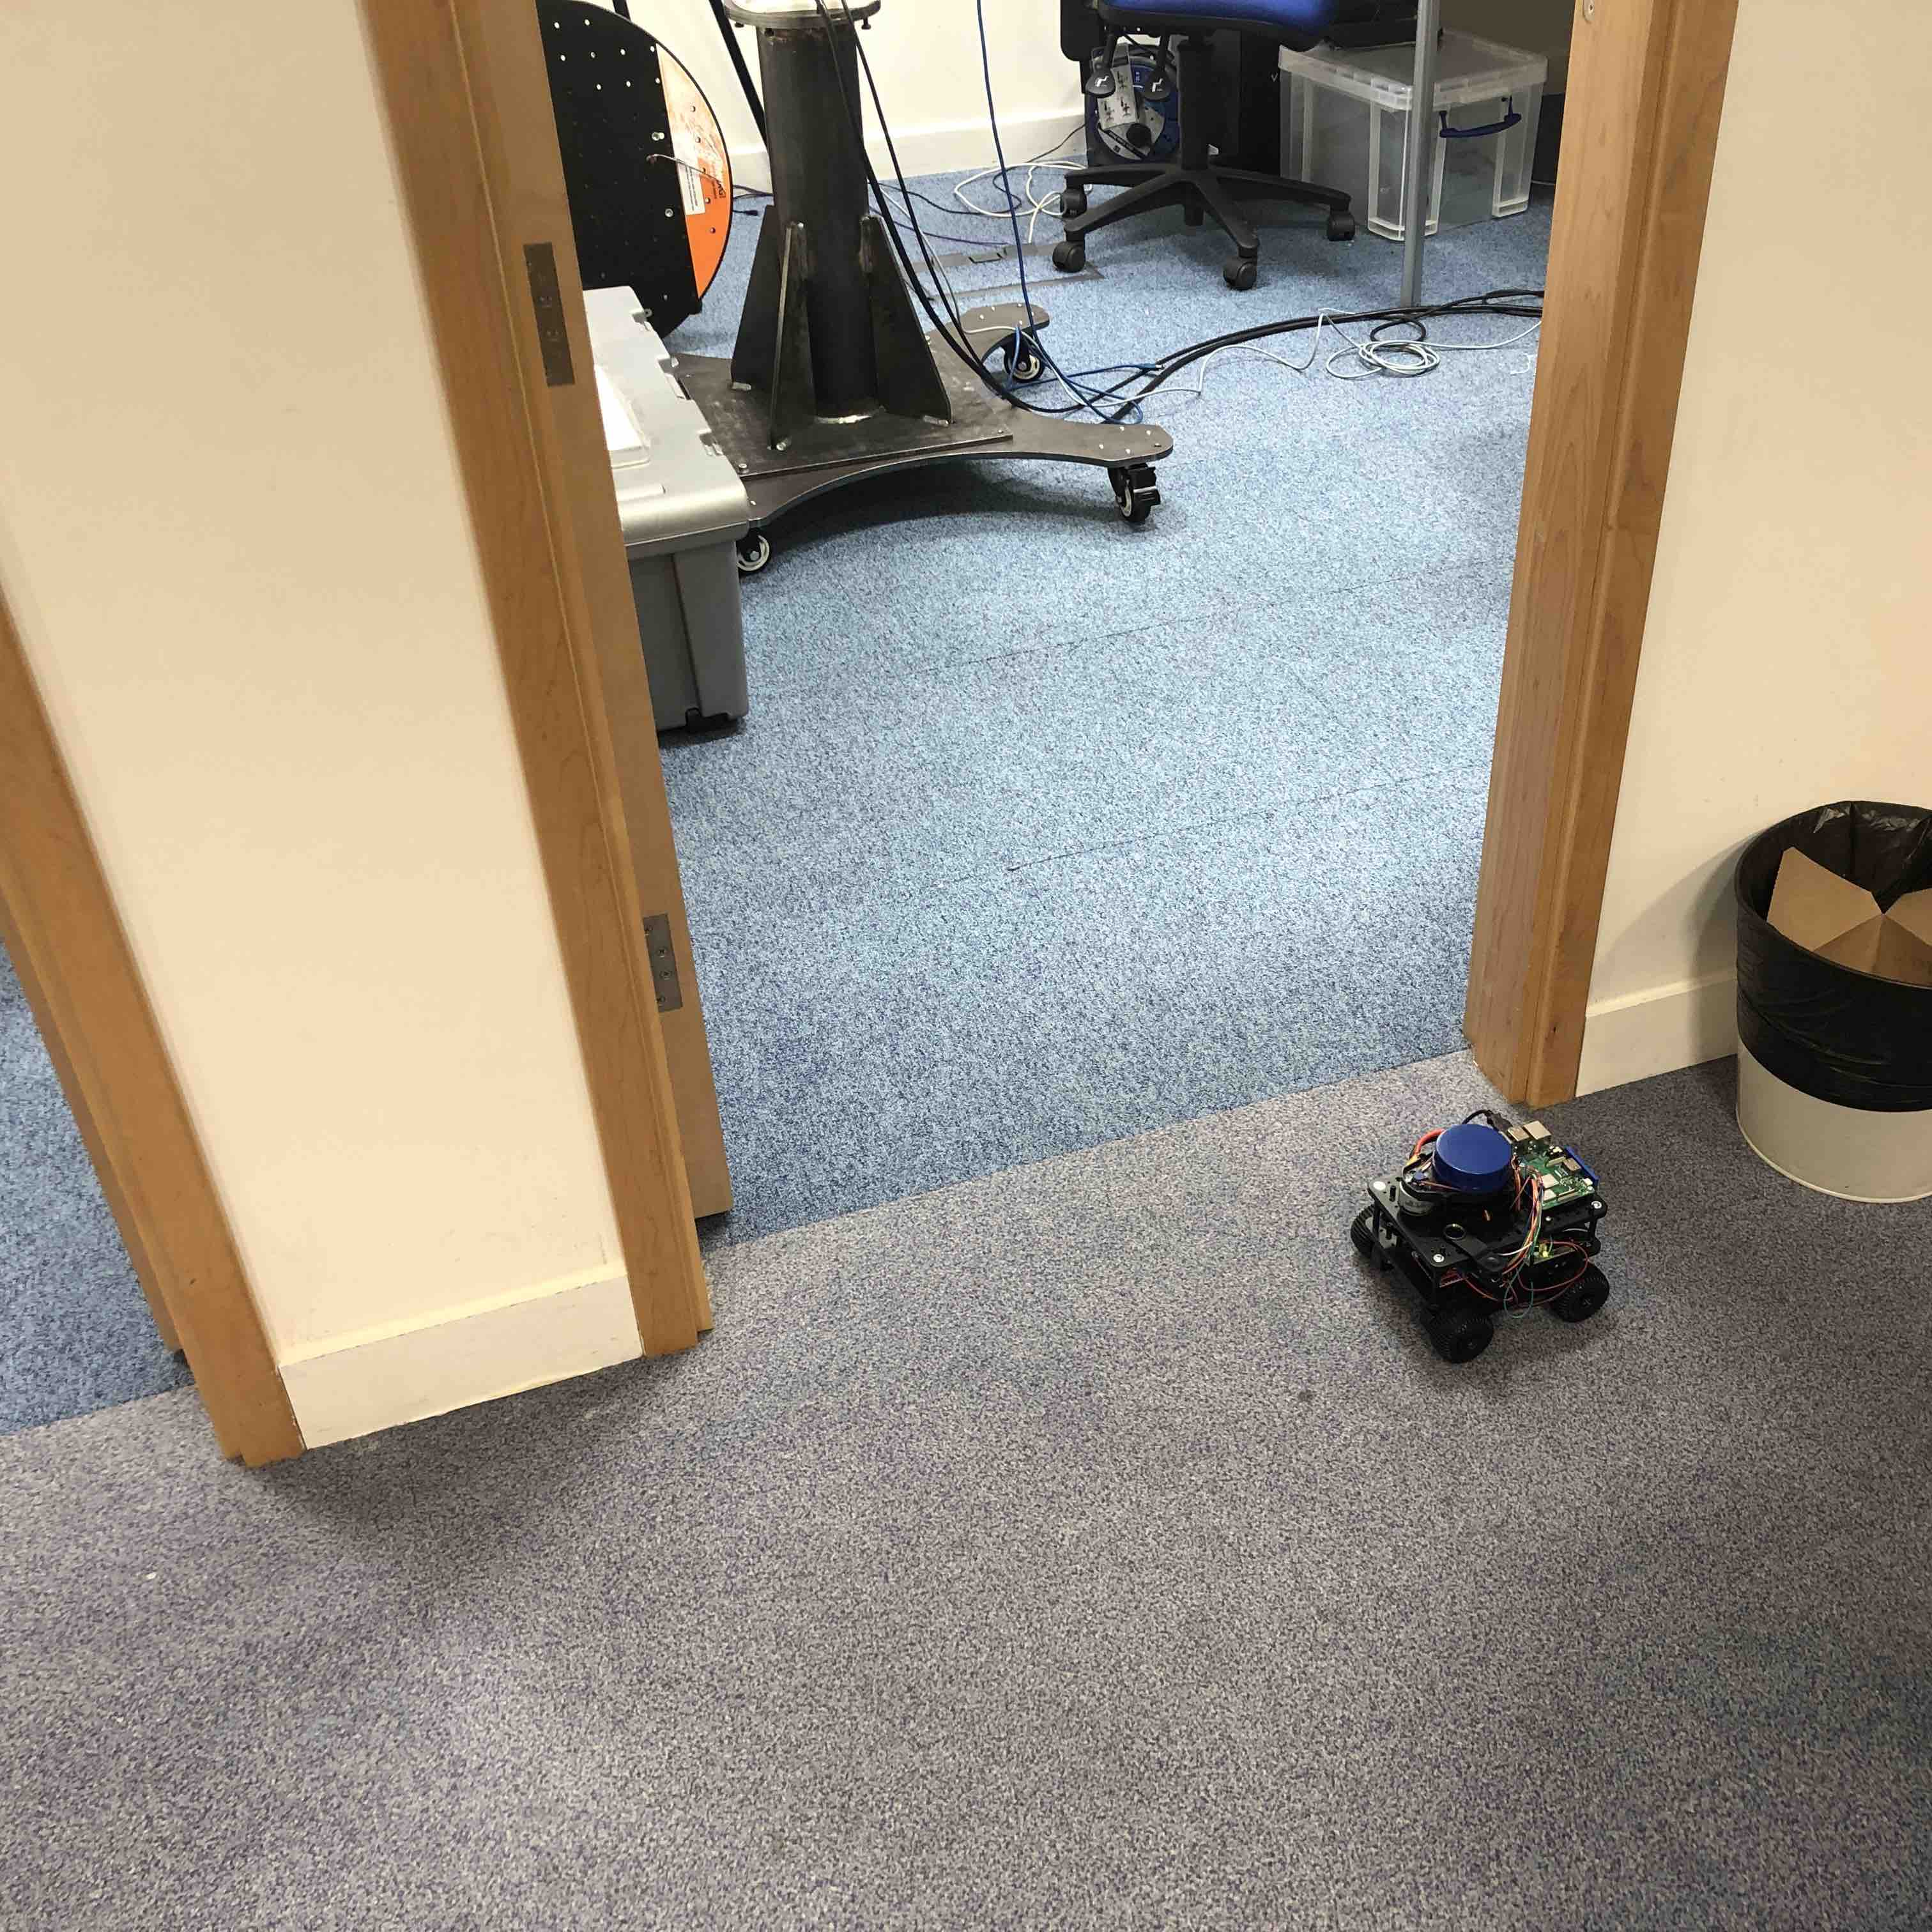
\includegraphics[width=\linewidth]{images/real/robo/4.JPG}
     \caption{Real-world: Reached WP 2}
  \end{subfigure}
  \hfill
  \begin{subfigure}[b]{0.32\linewidth}
    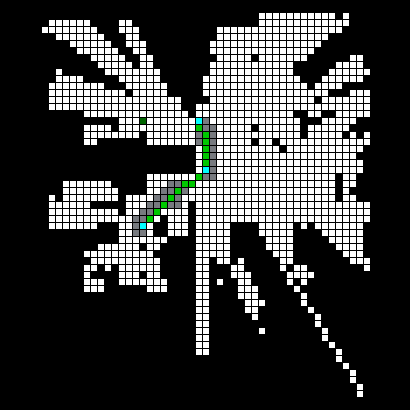
\includegraphics[width=\linewidth]{images/real/sys/4_2.png}
     \caption{PathBench: Reached WP 2}
  \end{subfigure}
  \hfill
  \begin{subfigure}[b]{0.32\linewidth}
    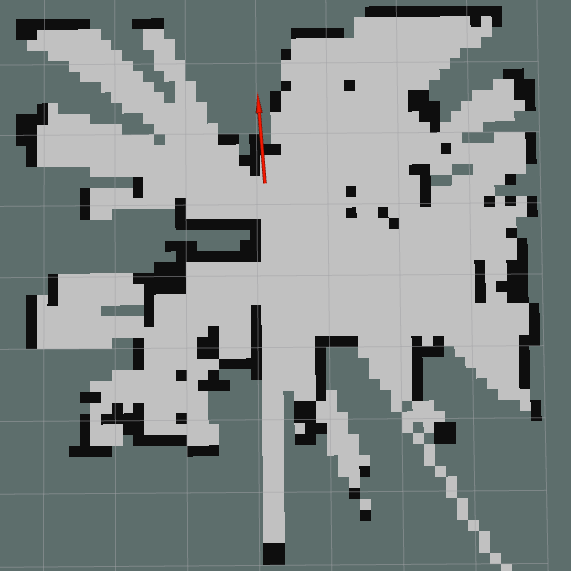
\includegraphics[width=\linewidth]{images/real/sys/4_3.png}
     \caption{Rviz: Reached WP 2}
  \end{subfigure}
  
  \newline
  
  \begin{subfigure}[b]{0.32\linewidth}
    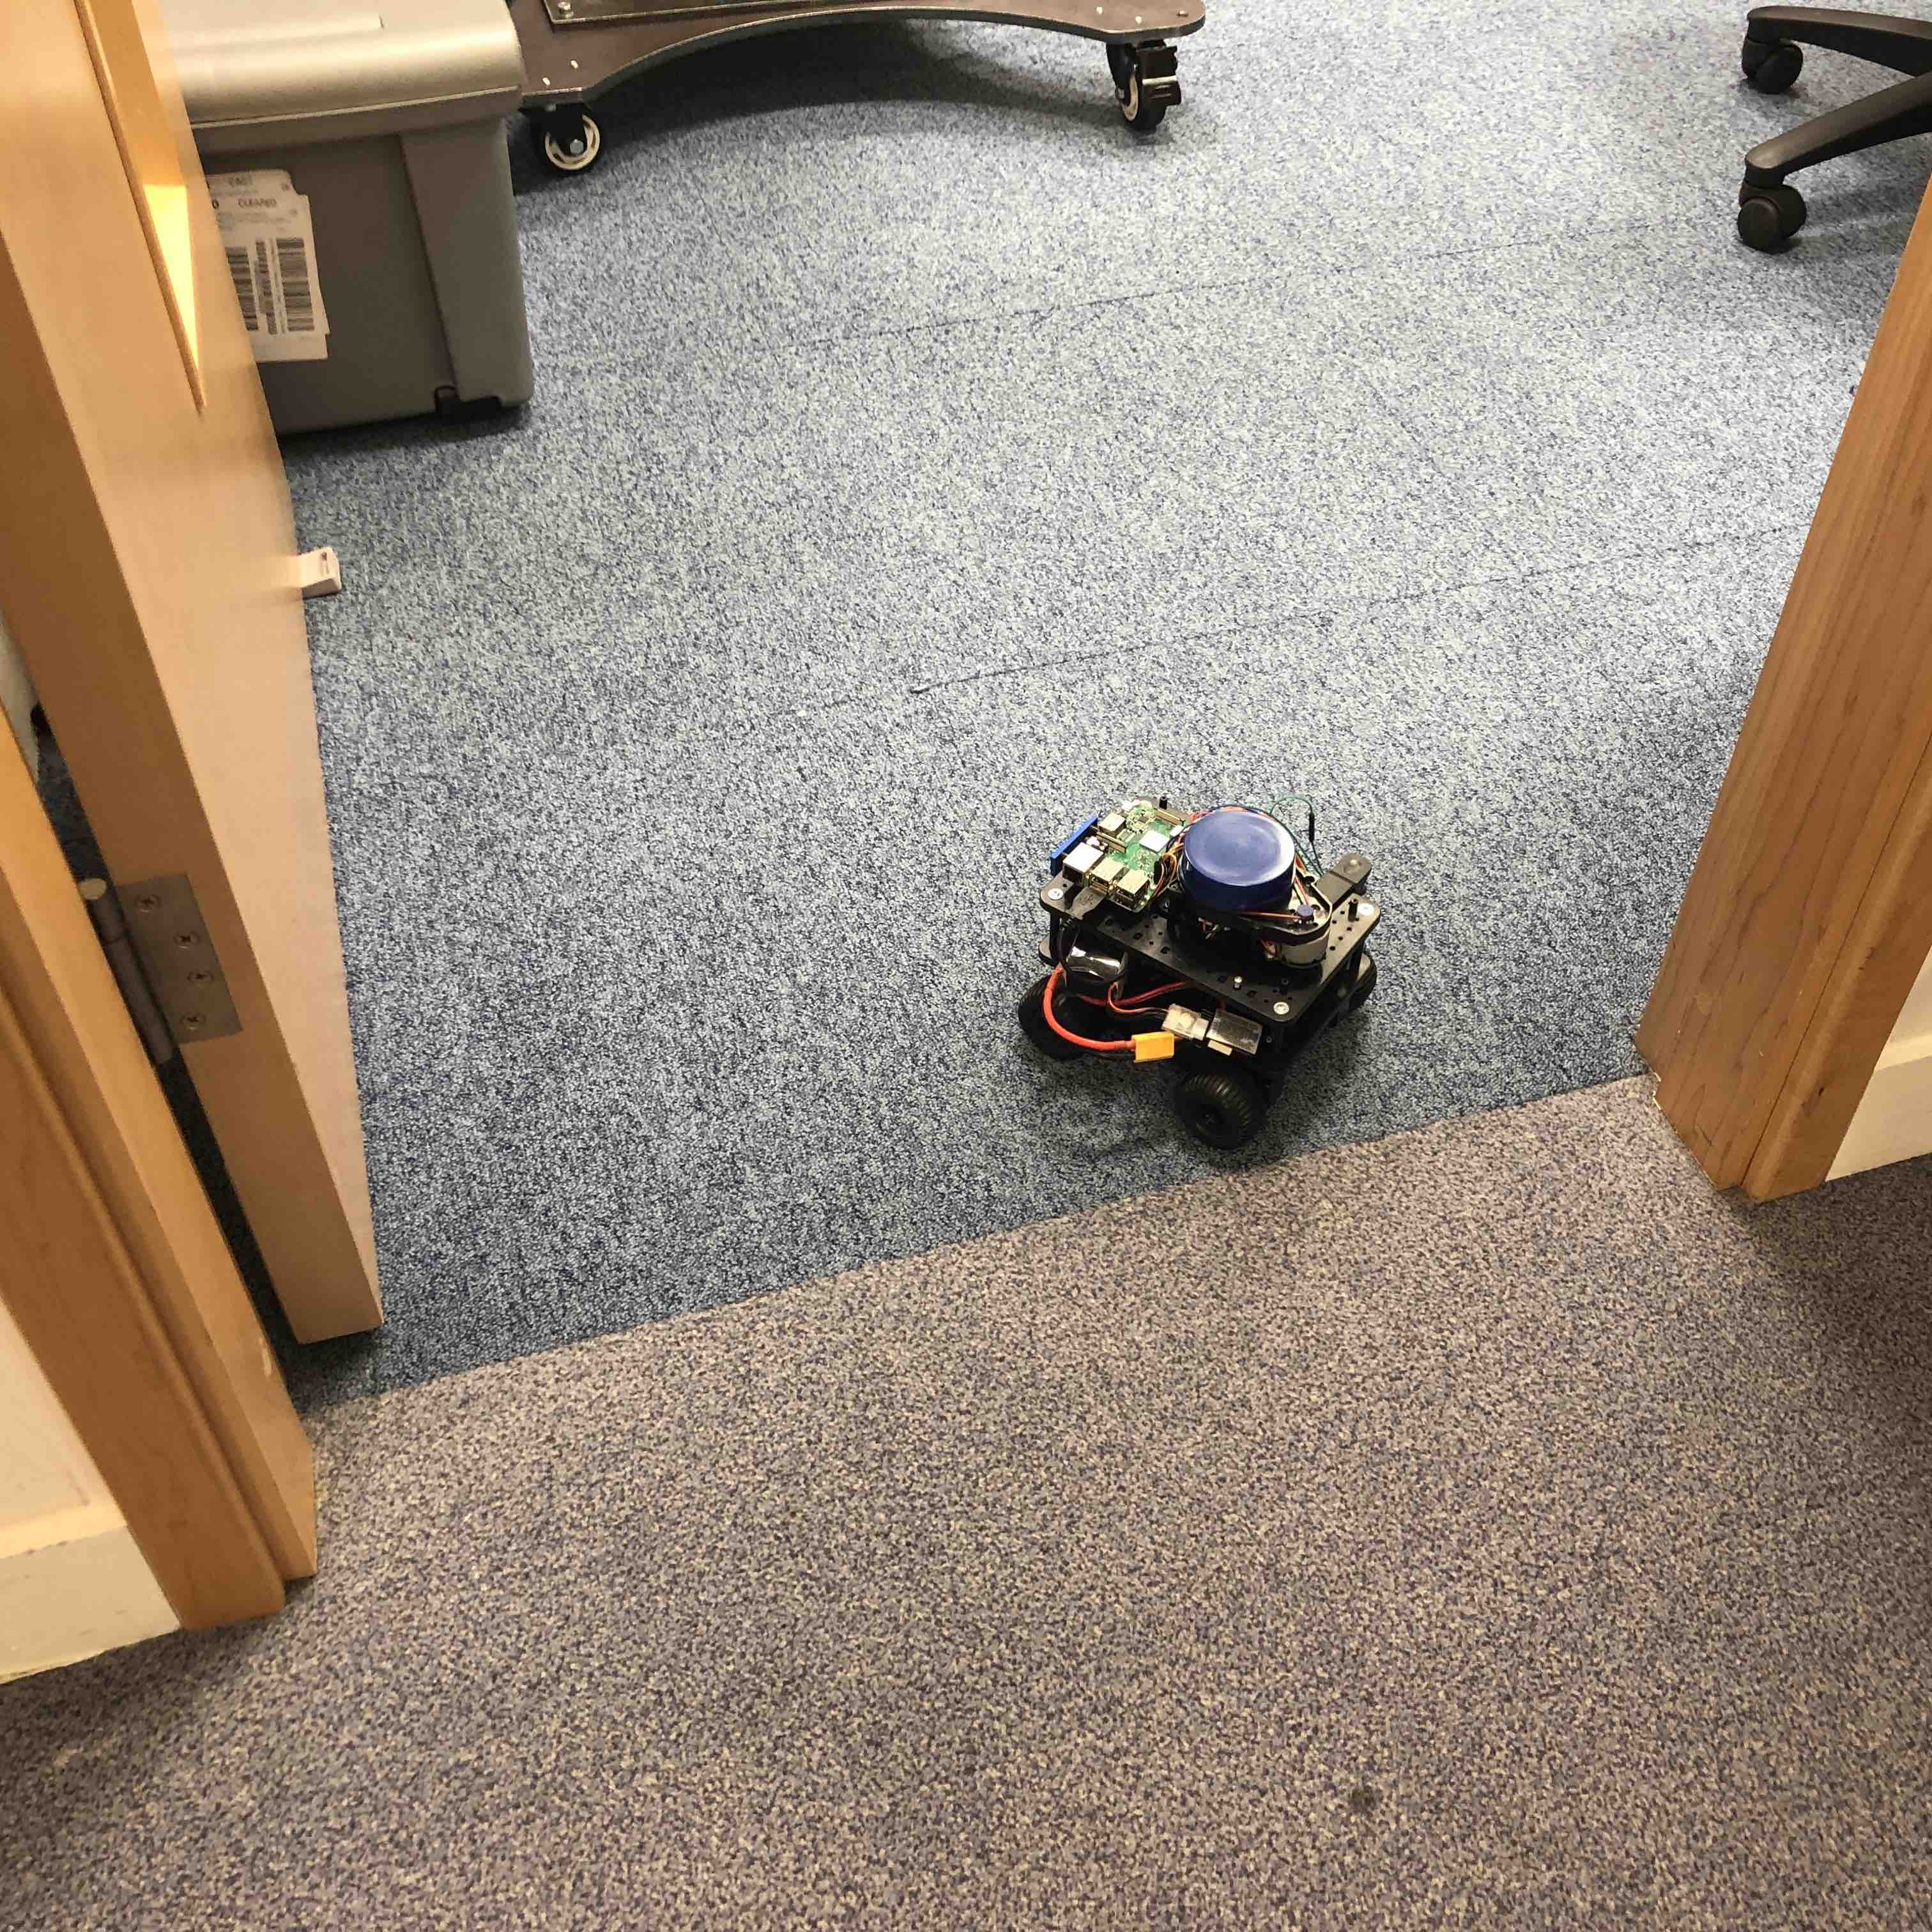
\includegraphics[width=\linewidth]{images/real/robo/5.JPG}
     \caption{Real-world: Suggested WP 3}
  \end{subfigure}
  \hfill
  \begin{subfigure}[b]{0.32\linewidth}
    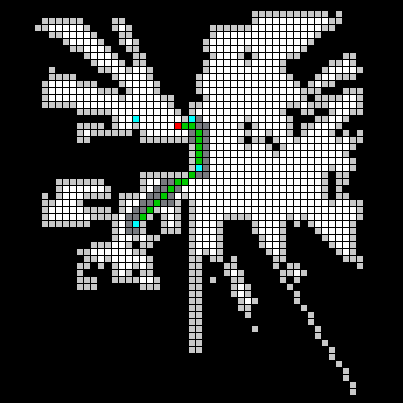
\includegraphics[width=\linewidth]{images/real/sys/5_2.png}
     \caption{PathBench: Suggested WP 3}
  \end{subfigure}
  \hfill
  \begin{subfigure}[b]{0.32\linewidth}
    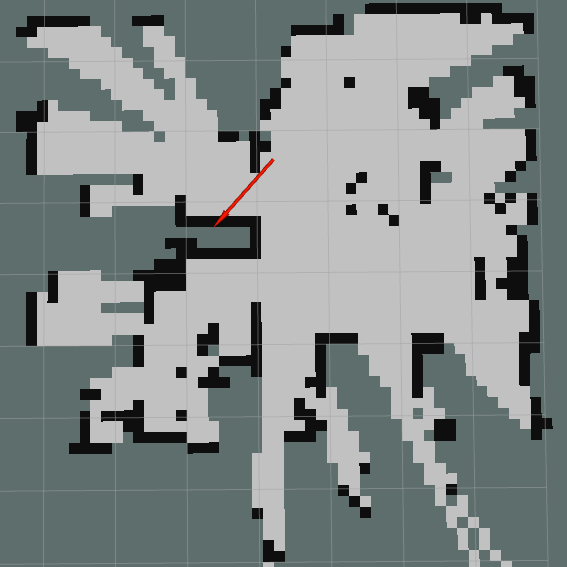
\includegraphics[width=\linewidth]{images/real/sys/5_3.png}
     \caption{Rviz: Suggested WP 3}
  \end{subfigure}
  
  \newline
  
  \begin{subfigure}[b]{0.32\linewidth}
    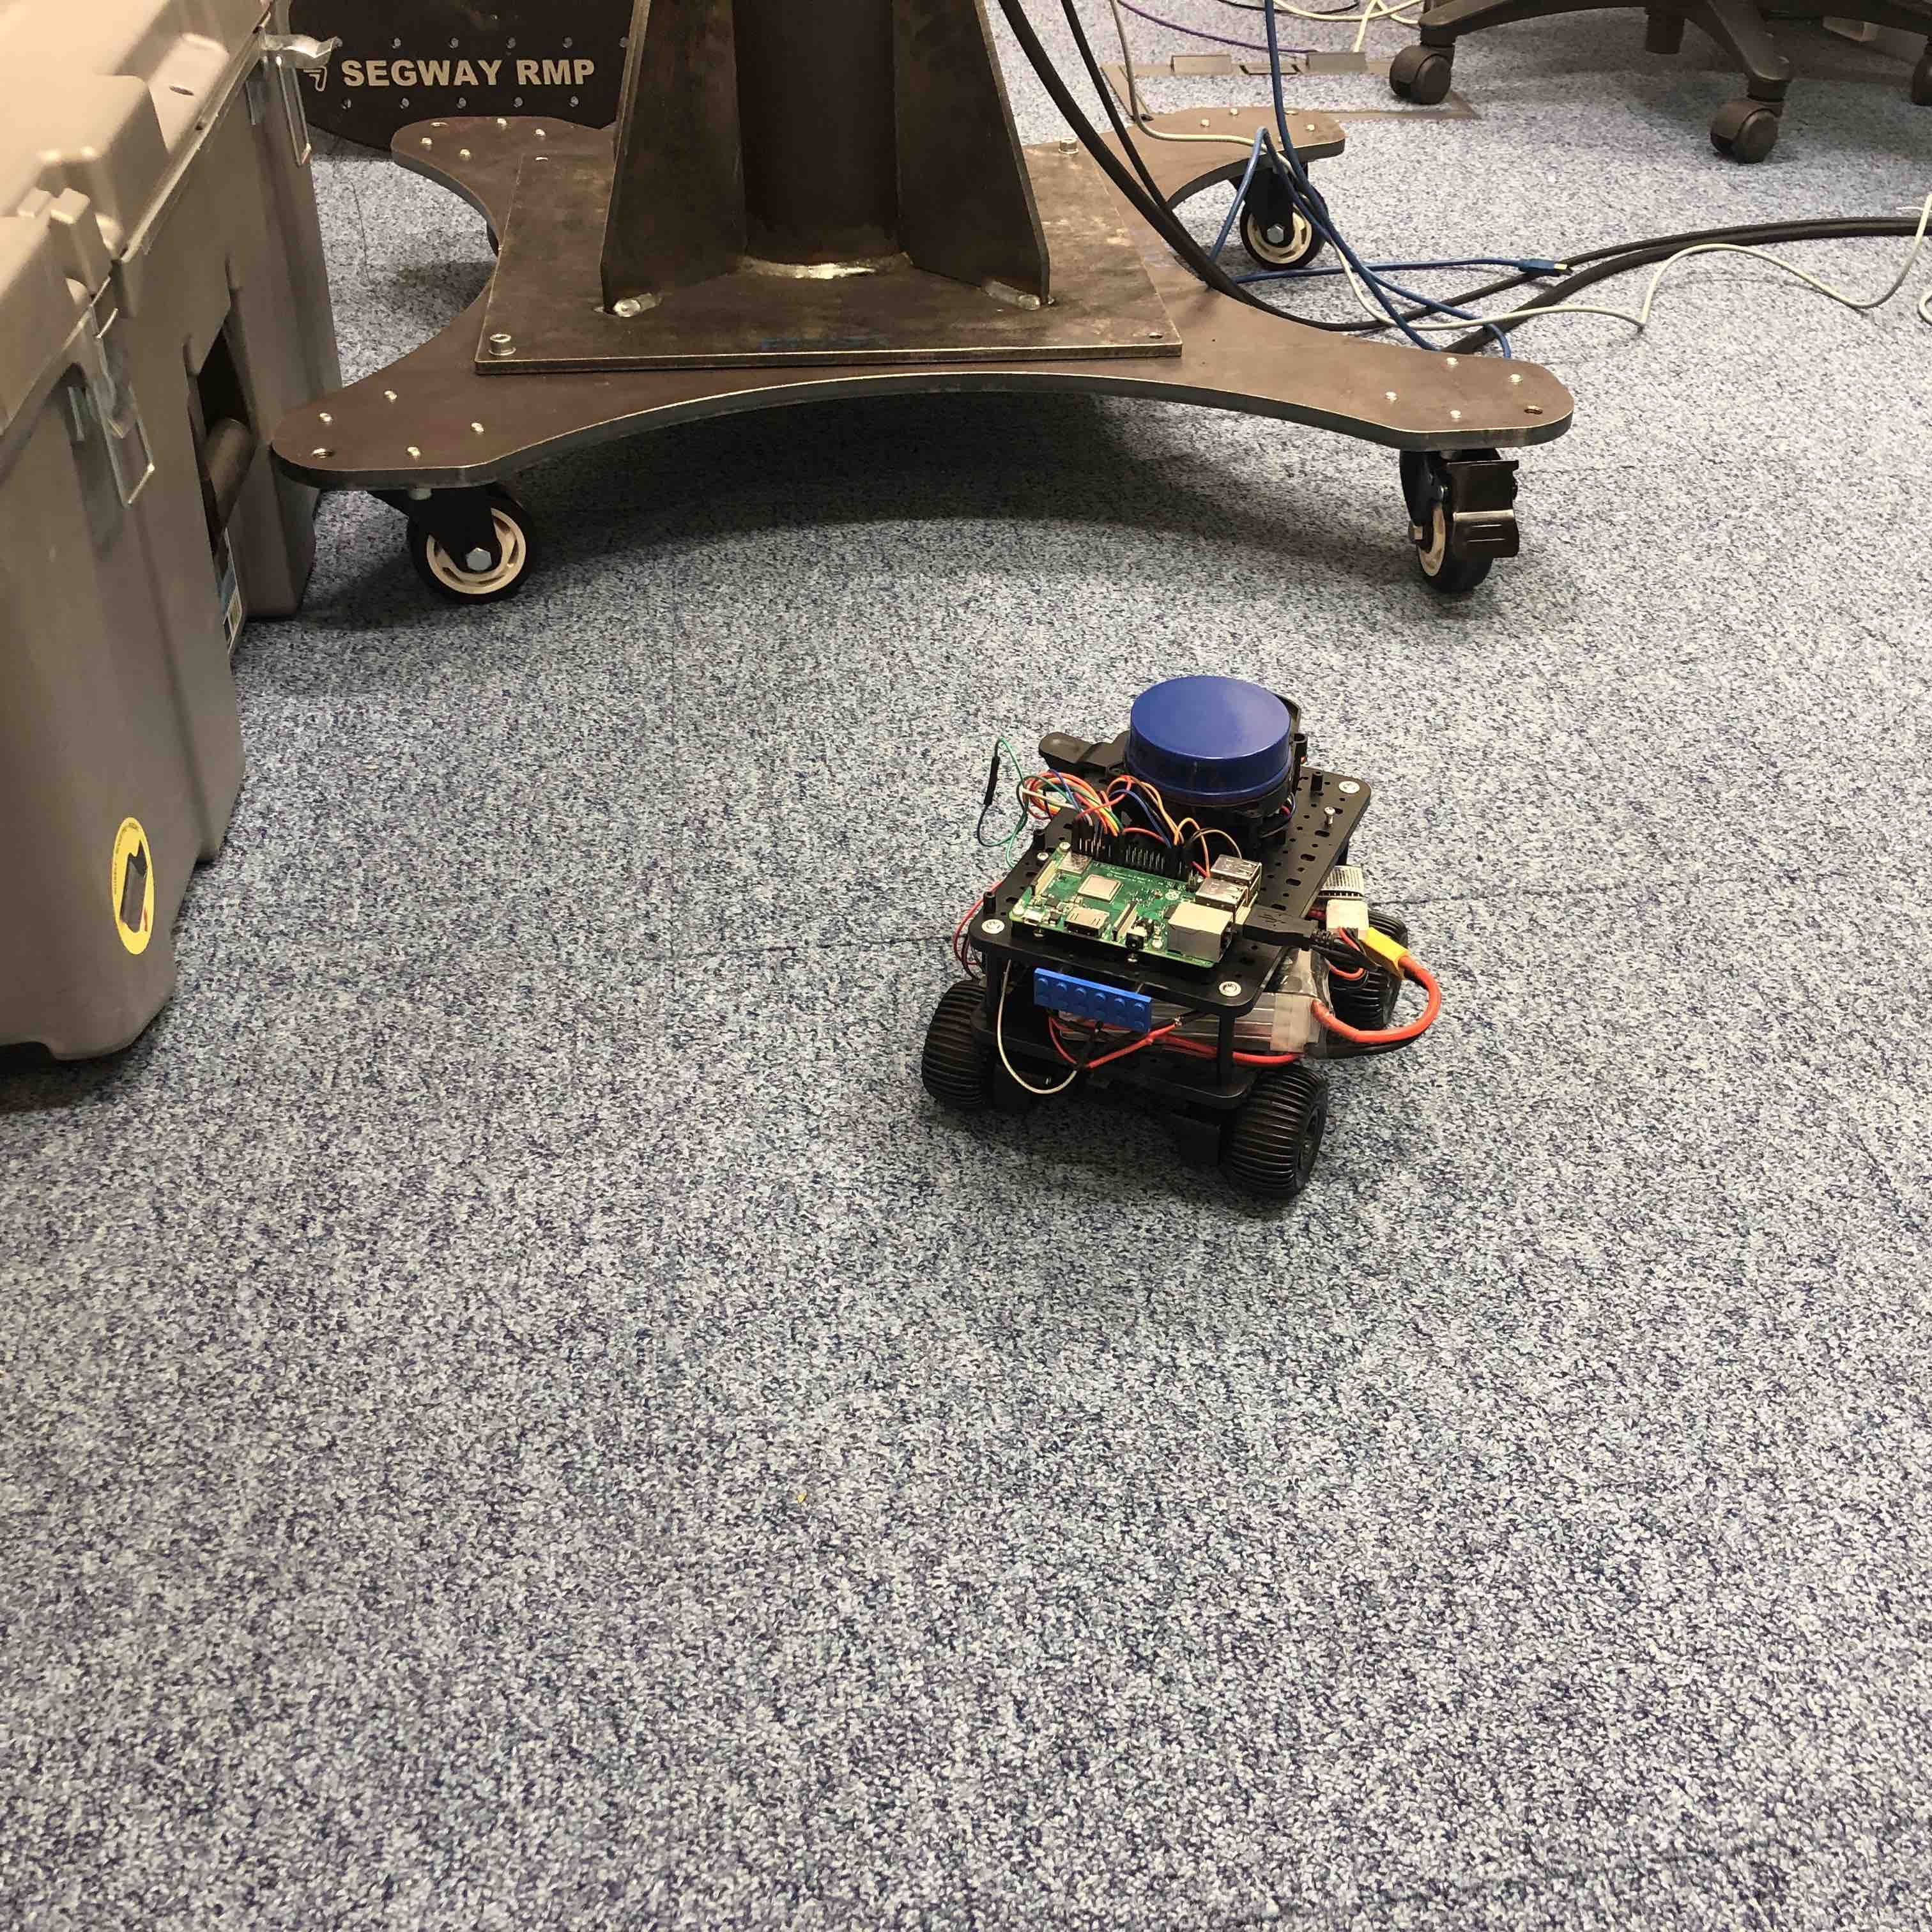
\includegraphics[width=\linewidth]{images/real/robo/final}
     \caption{Real-world: Final}
  \end{subfigure}
  \hfill
  \begin{subfigure}[b]{0.32\linewidth}
    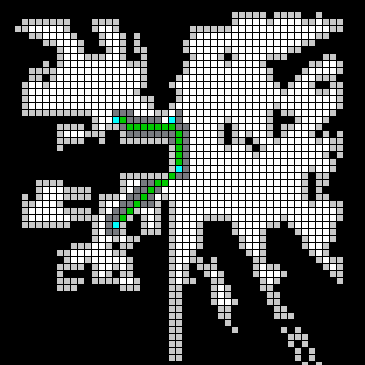
\includegraphics[width=\linewidth]{images/real/sys/final_2.png}
     \caption{PathBench: Final}
  \end{subfigure}
  \hfill
  \begin{subfigure}[b]{0.32\linewidth}
    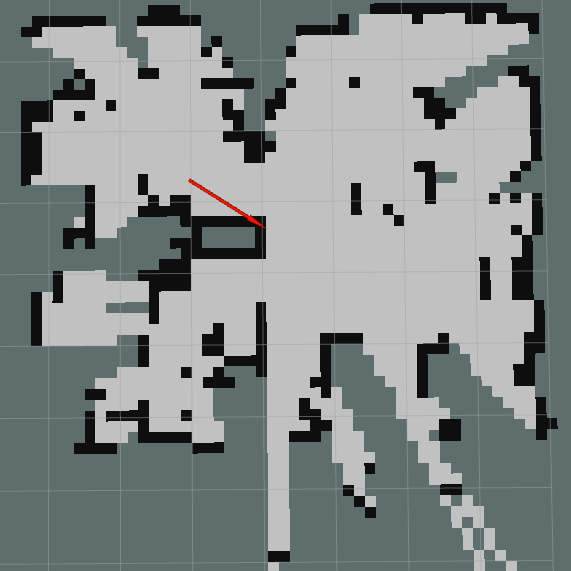
\includegraphics[width=\linewidth]{images/real/sys/final_3.png}
     \caption{Rviz: Final}
  \end{subfigure}
  
  \caption{Robot Path Planning using Global Way-point LSTM Planner run on the trajectory from Figure \ref{fig: robot}. The left image represents real-word view of the robot, the center image represents our live PathBench simulator visualisation and the right image represents the live Rviz simulator from ROS. The PathBench and Rviz images are cropped so that we only show the relevant information. The true dimension of the grid is $128 \times 128$}
  \label{fig: robot_run}
\end{figure}

\clearpage

\begin{table}[h!]
    \centering
    \begin{tabular}{|c|M{6.2cm}|}
         \hline
         \textbf{Name} & \textbf{Value} \\
         \hline
         Goal Found & \texttt{True} \\
         \hline
         Grid Cell Size & 0.15 meters \\
         \hline
         Map Size & $128 \times 128$ \\
         \hline
         Obstacles & 92.03\% \\
         \hline
         Original Distance & 15.00/2.25 meters \\
         \hline
         Distance & 28.56/4.824 meters \\
         \hline
         Time & 365.252545 seconds/6.08 minutes \\
         \hline
         Distance Left & 0.00/0.00 meters \\
         \hline
         Pick Ratio & [0.0\%, 33.33\%, 33.33\%, 0.0\%, 0.0\%, 33.33\%, 0.0\%, 0.0\%, 0.0\%, 0.0\%] \\
         \hline
         GK Improvement & 100.00\% \\
         \hline
         GK Distance & 28.56/4.824 meters \\
         \hline
         GK Distance Left & 0.00/0.00 meters \\
         \hline
         WP & \texttt{4} \\
         \hline
         WP In-Between Distance & 9.04/1.356 meters \\
         \hline
         Total Search & 0.47\% \\
         \hline
         Total Fringe & 0.31\% \\
         \hline
         Session Search & 0.13\% \\
         \hline
         Session Fringe & 0.09\% \\
         \hline
    \end{tabular}
    \caption{Reported real-world statistics on the run from Figure \ref{fig: robot_run}. The PathBench and Rviz images from Figure \ref{fig: robot_run} are cropped so that we only show the relevant information. The true dimension of the grid is $128 \times 128$}
    \label{tab: robot_stats}
\end{table}

The results show that the robot successfully found a path in a partial knowledge environment (See Figure \ref{fig: robot_run}) by placing the last global way-point on the goal. The evaluation metrics reported in Table \ref{tab: robot_stats} show that we retain the same behaviour discussed in the \textbf{Analyser} simple and complex routines (maximal GK Improvement, low number of way-points with high way-point in-between distance; it should be noted that time statistic is influenced by the speed of the robot). Therefore, we have shown that the Global Way-point LSTM Planner supports partial knowledge environments in which classic offline solutions such as A* are unable to find a path to the goal without making use of an exploration method. Lastly, we have showed that the simulator is compatible with the \textit{gmapping} \textit{ROS} package and has support for live updates.